\documentclass{article}
\usepackage{titlesec}

\usepackage[left=4cm, right=4cm]{geometry}
\usepackage{palatino}%Font
\usepackage{graphicx}
\usepackage{wrapfig}
\usepackage{float}
\usepackage{subcaption}
\usepackage{enumerate}
\usepackage{parskip}
\usepackage{multirow}
\usepackage{multicol}
\setlength{\columnsep}{-50pt}
\usepackage{listings}
\lstset{basicstyle=\ttfamily,
	breaklines=true}
\usepackage{fancyvrb}
\usepackage{booktabs}
\usepackage{amsthm}
\usepackage{amssymb}
\usepackage{amsmath}
\usepackage[htt]{hyphenat}
\usepackage{cancel}
\usepackage{tikz}
\usepackage{tikz-cd}
\usepackage{tikz-3dplot}
\usepackage{xcolor}
\usepackage[bookmarks,bookmarksopen,bookmarksdepth=3]{hyperref}
\hypersetup{
	colorlinks=true,
	urlcolor=blue,
	linkcolor=magenta,
	citecolor=blue,
	filecolor=blue,
	urlbordercolor=white,
	linkbordercolor=white,
	citebordercolor=white,
	filebordercolor=white
}

\usepackage{etoolbox}
\usepackage{cleveref}
\crefname{figure}{fig.}{figs.}
\Crefname{figure}{Fig.}{Figs.}
\renewcommand{\figurename}{Fig.}
\usepackage{appendix}

%Bold references
%\usepackage{xpatch}
%\makeatletter
%\xpatchcmd{\@cref}{\begingroup}{\begingroup\bfseries}{}{}
%\makeatother
%\captionsetup[figure]{labelfont=bf}

\theoremstyle{definition}

\newtheorem*{defn}{Definition}
\newtheorem*{lem}{Lemma}
\newtheorem*{rem}{Remark}
\newtheorem*{thm}{Theorem}
\newtheorem*{prop}{Proposition}
\newtheorem*{claim}{Claim}

\newcommand{\E}{\mathbb{E}}
\newcommand{\R}{\mathbb{R}}
\newcommand{\Z}{\mathbb{Z}}
\newcommand{\N}{\mathbb{N}}
\newcommand{\C}{\mathbb{C}}
\newcommand{\Q}{\mathbb{Q}}
\newcommand{\s}{\mathbb{S}}
\newcommand{\PP}{\mathbb{P}}
\newcommand{\p}{\mathcal{P}}
\newcommand{\T}{\mathcal{T}}
\DeclareMathOperator{\Id}{Id}
\DeclareMathOperator{\img}{img}
\DeclareMathOperator{\Fix}{Fix}
\DeclareMathOperator{\Stab}{Stab}

%Referencias
\usepackage[style=nature,backend=bibtex]{biblatex}
\addbibresource{bib.bib}

\title{A new chiral 4-polytope}
\author{\\Daniel González Casanova Azuela}
\date{}

\def\changemargin#1#2{\list{}{\rightmargin#2\leftmargin#1}\item[]}
\let\endchangemargin=\endlist

\begin{document}
\thispagestyle{empty}
\begin{figure}[H]
	\centering
	
\includegraphics[width=0.3\linewidth]{fig0}
\end{figure}

\begin{center}
	\textbf{UNIVERSIDAD NACIONAL AUTÓNOMA DE MÉXICO}
	
	PROGRAMA DE MAESTRÍA Y DOCTORADO EN CIENCIAS MATEMÁTICAS Y DE LA ESPECIALIZACIÓN EN ESTADÍSTICA APLICADA
	
	\vspace{2cm}
	{\Large Two new chiral 4-polytopes in $\E^4$}
	\vspace{1.2cm}
	
	TESINA
	
	QUE PARA OPTAR POR EL GRADO DE:
	
	MAESTRO EN CIENCIAS
	\vspace{1.2cm}
	
	PRESENTA:
	
	DANIEL GONZÁLEZ CASANOVA AZUELA
	\vspace{1.2cm}
	
	DIRECTOR:
	
	JAVIER BRACHO CARPIZO
	
	INSTITUTO DE MATEMÁTICAS, UNAM
	\vspace{1.2cm}
	
	LUGAR, MES Y AÑO
\end{center}

\clearpage

\begin{changemargin}{3.3cm}{0cm} 
%\section*{Agradecimientos}

\vspace*{4cm}

{\Large\textbf{Agradecimientos}}
\vspace{1cm}

A mis queridos tutores Roli e Isabel por transmitirme tanta emoción. A Bris por ser un modelo a seguir. Al equipo de politoperes por todo su cariño. A Vinicio Gómez por estar siempre. A mi familia.
\end{changemargin}
\clearpage
	
	
	\section*{Summary}
	In the context of skeletal geometric complexes, chiral polytopes are those with maximal rotational symmetry but no reflection symmetry. We construct a chiral 4-polytope in $\E^4$ by choosing three orientation-preserving isometries within the symmetry group of the regular star 4-polytope $\left\{\frac{5}{2},3,5\right\}$. Chirality follows from the cells' chirality, which are copies of the polyhedron $H_1(\left\{5,3,\frac{5}{2}\right\})$ from \cite{petcox}. Analogue choices of isometries within the symmetry group of the dual $\left\{5,3,\frac{5}{2}\right\}$ are shown to produce a similar chiral 4-polytope. Both polytopes are shown to be combinatorially chiral.
	
	\vspace{1cm}
	%	\phantomsection
		\tableofcontents
		\clearpage
	\section{Introduction}
	Despite polygons and polyhedra being basic concepts in mathematics,
	% studied since antiquity,
	 it is not at all obvious what exactly these words mean. Chiral polytopes arise from the so-called skeletal approach, where polygons and their higher-dimensional analogues are introduced as 1-dimensional complexes, with no need of an enclosed surface or solid.
	
	Such definition allows for symmetric structures otherwise unseen, an example of which are chiral polytopes. While the symmetry group of a regular polyhedron acts transitively on the set of flags, a polyhedron is geometrically chiral when its symmetry group has two orbits on the flags and adjacent flags are in distinct orbits. This captures the idea of maximal rotational symmetry but no reflection symmetry.
	
	Chiral polyhedra first appeared in 2005, when Schulte classified those realisable in $\E^3$, non of which is finite nor its faces are contained in planes (see \cite{chiral-polyhedra-i,chiral-polyhedra-ii}). The first example of a chiral 4-polytope in $\E^4$, so-called Roli's cube, was constructed in 2014 by Bracho, Hubard and Pellicer \cite{rolis-cube}. It was later shown that the facets of this polytope belong to a broader family of chiral polyehdra with helical faces in $\mathbb{S}^3$ \cite{petcox}.
	
	In this thesis we show that the natural rotation about an edge of two of such spherical polyhedra successfully yield, respectively, two new chiral 4-polytopes. Their combinatorial structures are then shown to be chiral as well---something that does not occur for their facets, which are combinatorially regular.
	
	Demostrations are given by GAP programs in which the abstract and geometric structures are compared. Geometric realizations are based on the reflection matrices used in \cite{petcox}. A wide range of figures created in Mathematica are provided, some of which use part of the code developed for the aforementioned paper. All programs used are available \href{https://github.com/danimalabares/tesina.git}{online}.
	
	\section{Historical background}
	We begin with a brief historical discussion on the concept of polytope.
	
	We cannot find a moment in history when triangles and squares came to attract the attention humans. Later, when mathematics became an established discipline, simple polygons polyhedra were thoroughly studied: the first proposition in Euclid's elements is the construction of a regular triangle, and the last book is devoted to the study of Platonic Solids \cite{euclid}.
	
	After the greeks, the definition of polygon remained essentialy unchanged for many centuries. The first account of an important difference dates to the XIV century, when an Archbishop of Canterbury investigated star polygons \cite{abstract-polytopes}.
	These are essentially different by being non-convex: their edges intersect in points that are not vertices of the polygon. They may be, however, studied by their symmetry properties just like regular convex polygons.
	
	Regular star polyhedra are the natural generlization of regular star polygons to euclidean 3-space. They take us to the XVII century with Johannes Kepler, who studied the two whose faces are star polygons (pentagrams). Their duals, whose faces are convex but their vertex-figures are not, where studied in 1809 by Louis Poinsot \cite{abstract-polytopes}.
	
	The first time higher-dimensional polytopes were studied was in the XIX century, when Ludwig Schläfli found all the regular polytopes whose symmetry groups are generated by reflections in hyperplanes in euclidean spaces \cite{abstract-polytopes}.
	
	Next in history is Coxeter, who, among many other results, classiffied all discrete euclidean reflection groups. In the 1930's him and Petrie redefined further the concept of polytope by letting them have infinite faces, thus finding three more regular polyhedra in $\E^3$ \cite{regular-skew}. These have non-planar vertex figures.
	
	Fourty years later, in 1977, Grünbaum once again reintroduced polytopes, this time letting even the faces be non-planar \cite{grunbaum}. The list of regular polyhedra in $\E^3$ was extended to 18 in the finite case and 48 in total \cite{regular-ordinary}. All but one were classified by Grünbaum, the remaining and the completeness of the list due to Dress \cite{Dress1981,Dress1985}.
	
	The study of the underlying combinatorial structure of polytopes led to the concept of abstract polytope. In 1967 McMullen studied the lattice of faces of a polytope and compared its automorphisms with geometric symmetries \cite{mcmullen-combinatorially}. In Grümbaum's \cite{grunbaum-regularity}, the term \textit{polystroma} (stroma=stratum, layer) is defined to mean an abstract partially order structure resembling the face lattice of a polytope.
	
	Chiral polytopes were first studied in this abstract sense, a general theory first given in 1991 by Schulte and Weiss \cite{schulte-chiral}. Back to geometry, skeletal chiral polyhedra in $\E^3$ were studied in \cite{chiral-polyhedra-i,chiral-polyhedra-ii}, and the first example of a skeletal chiral 4-polytope in $\E^4$ is Roli's cube from \cite{rolis-cube}.
	
	\section{Skeletal polyhedra and 4-polytopes in $\E^4$}\label{sec:skeletal}
	Now we give formal definitions and basic results.
	
	A \textit{skeletal polyhedron} in $\E^4$ consists of \textit{vertices} (points in $\E^4$), \textit{edges} (segments between vertices) and \textit{faces} (cycles of the vertices) such that:
	\begin{enumerate}[\itshape(i)]
		\item every edge belongs to two faces,
		\item the graph determined by the vertices and edges is connected,
		\item every compact subset of $\E^4$ meets finitely many edges, and
		\item the \textit{vertex-figure}, defined as follows, is a connected graph. For any vertex $v$, the vertices of the vertex-figure are the neighbours of $v$ and the edges are segments joining any two neighbours that are both in some face.
	\end{enumerate}
	A \textit{skeletal 4-polytope} in $\E^4$ consits of vertices, edges, faces and \textit{cells} (skeletal polyhedra on the set of vertices, edges and faces), such that
	\begin{enumerate}[\itshape(i)]
		\item every face belongs to two cells,
		\item the graph determined by the vertices and the edges is connected,
		\item every compact subset of $\E^4$ meets finitely many edges, and
		\item the vertex-figure at every vertex is a skeletal polyhedron.
		\end{enumerate}
	
	Hereafter we omit the term "skeletal" from our definition. If $\p$ is a 4-polytope, the set of vertices, edges, faces and cells is a partial order with respect to inclusion. We say two such elements are \textit{incident} if they are comparable. This poset is called the \textit{abstract polytope associated to $\p$}. As we shall see, 4-polytopes defined as above are \textit{realizations} of abstract polytopes in the sense of \Cref{sec:abstract-defs}.
	
	A \textit{flag} is a 4-tuple of incident vertex, edge, face and cell. Two flags are \textit{adjacent} when they differ by only one element. We call two flags \textit{0-adjacent} if they difer by a vertex, \textit{1-adjacent} if they difer by an edge, \textit{2-adjacent} if they difer by a face and \textit{3-adjacent} if they difer by a cell.
	
	A \textit{symmetry} of $\p$ is an isometry of $\E^4$ that preserves it set-wise. The group of symmetries of $\p$ will be denoted by $G(\p)$. We call $\p$ \textit{regular} if $G(\p)$ acts transitively on the set of flags, and \textit{chiral} if $G(\p)$ induces two orbits on flags so that adjacent flags are on different orbits. In fact, whether $\p$ is regular or chiral, its symmetry group acts transitively on the sets of vertices, edges, faces and cells.
	

	
\section{Abstract 4-polytopes}\label{sec:abstract-defs}
	The theory of abstract polytopes is an essential tool for our work. In this section we state basic results and constructions upon which our demonstrations hold.
	
	An \textit{abstract $4$-polytope} is a partial order $\p$ that satisfies properties \hyperref[P1,P2,P3,P4]{P1,P2,P3,P4}. The elements of $\p$ are called \textit{faces} and maximally ordered subsets (chains) are called \textit{(abstract) flags}. We require that
	\begin{enumerate}
		\item[(P1)]\label{P1} $\p$ contains a least face and a greatest face, denoted respectively by $F_{-1}$ and $F_4$.
		\item[(P2)]\label{P2} Flags contain $6$ elements, including $F_{-1}$ and $F_4$.
	\end{enumerate}
	Every element in a poset is in some chain, so that we may assign to every face a number from $-1$ to $4$. Such is the \textit{rank function} of $\p$. We say two flags are \textit{$i$-adjacent} if they differ only by a face of rank $i$.
	\begin{enumerate}
		\item[(P3)]\label{P3} $\p$ is \textit{strongly flag connected} in the following sense. For any two distinct flags $\Phi$ and $\Psi$ there is a sequence
		\[\Phi=\Phi_0,\Phi_1,\ldots,\Phi_k=\Psi\]
		so that $\Phi_{i-1}$ and $\Phi_i$ are adjacent and $\Phi\cap\Psi\subset\Phi_i$ for all $i$.
		\item[(P4)]\label{P4} If $F$ and $G$ are a $(i-1)$-face and a $(i+1)$-face with $F<G$ and $0\leq j\leq2$, then there are exactly two $i$-faces $H$ such that $F<H<G$.
	\end{enumerate}
	
		\subsection{Regular and chiral abstract 4-polytopes}
	Now we study regular 4-polytopes and their automorphism groups. An \textit{automorphism} of $\p$ is a bijection of the abstract polytope that preserves incidence, and we denote automorphism group by $\Gamma(\p)$. A an abstract polytope is called \textit{regular} if $\Gamma(\p)$ is transitive on flags.
	
	For a regular polytope $\p$ and some distinguised flag $\Phi$, there exists a unique involutory automorphism $\rho_j$ of $\p$ such that $\Phi\rho_i=\Phi^i$ for $i=0,1,2,3$ (Prop. 2B4, \cite{abstract-polytopes}). These are called the \textit{distinguished generators} of $\Gamma(\p)$ and satisfy that $(\rho_i\rho_j)^{p_{ij}}=\Id$ for $i,j=0,1,2,3$. The numbers $p_i:=p_{i-1}p_i$ form the \textit{Schläfli type} $\{p_1,p_2,p_3\}$ of $\p$ and its automorphism group is denoted by $[p_1,p_2,p_3]$.
	
	In fact, if $\p$ is regular, $\Gamma(\p)$ is a C-string group in the following sense (props. 2B10 and 2B11, \cite{abstract-polytopes}). Let $\Gamma$ be a group generated by the involutions $\rho_0,\rho_1,\rho_2,\rho_3$. We say $\Gamma$ is a \textit{C-string group} if
	\[(\rho_i\rho_j)^2=\Id\text{ when } |i-j|\geq2\]
	and it has the \textit{intersection property}, namely
	\[\langle \rho_i|i\in I\rangle\cap\langle\rho_j|j\in J\rangle=\langle\rho_i\in I\cap J\rangle\qquad\text{for }I,J\subseteq\{1,2,3\}.\]
	%	An polyhedron is called \textit{equivelar} if every face has the same number of edges $p$ and every vertex has the same degree $q$. We say that the \textit{Shläfli type} of $\p$ is $\{p,q\}$.
	%	
	%	Analogously, a 4-polytope $\p$ is \textit{equivelar} it every face has the same number of edges, every vertex the same degree, and every edge
	%	
	Conversely, we may construct a regular abstract $4$-polytope from a C-string group $\Gamma$. Define $\Gamma_j:=\langle\rho_j|i\neq j\rangle$ and $\Gamma_{-1}=\Gamma_4:=\Gamma$, and take the set of $i$-faces to be the set of right cosets $\Gamma_i\varphi$ for $\varphi\in\Gamma$. Then this set admits an order relation with respect to which it is a regular $4$-polytope whose automorphism group is $\Gamma$ (thm. 2E11, \cite{abstract-polytopes}).
	
	\vspace{.5cm}
	
	Now we revise the analogue construction for chiral polytopes. An abstract 4-polytope $\p$ is called \textit{chiral} if $\Gamma(\p)$ induces two orbits on flags and two adjacent flags are in different orbits.
	
	It turns out that by defining $\sigma_i:=\rho_{i-1}\rho_i$ for the distinguished generators of a regular polytope, it holds that
	\begin{equation}\label{eq:chiral-rels}
		\begin{aligned}
			\sigma_1^{p_1}=\sigma_2^{p_2}&=\sigma_3^{p_3}=\Id\\
			(\sigma_1\sigma_2)^2=(\sigma_1\sigma_2&\sigma_3)^2=(\sigma_2\sigma_3)^2=\Id
		\end{aligned}
	\end{equation}
	for some positive integers $p_1$, $p_2$ and $p_3$.
	
	The group generated by these elements is called the \textit{rotation subgroup} of $\p$, denoted by $\Gamma^+(\p)$. For chiral polytopes this will be the whole group: if $\p$ is chiral, $\Gamma(\p)$ is generated by three automorphisms $\sigma_1,\sigma_2$ and $\sigma_3$ that satisfy \cref{eq:chiral-rels} (prop. 3, \cite{schulte-chiral}).
	
	To construct a chiral or regular abstract polytope from a group we must also require some sort of intersection property. It will suffice that
	\begin{equation}\label{eq:chiral-int}
		\begin{aligned}
			\langle\sigma_1\rangle\cap\langle\sigma_2\rangle=\{\Id\}&=\langle\sigma_2\cap\langle\sigma_3\rangle\\
			\langle\sigma_1,\sigma_2\rangle\cap\langle\sigma_2,\sigma_3\rangle&=\langle\sigma_2\rangle
		\end{aligned}
	\end{equation}
	Let $\Gamma=\langle \sigma_1,\sigma_2,\sigma_3\rangle$ be a group satisfying both \cref{eq:chiral-rels,eq:chiral-int}. Define
	\begin{align*}
		\Gamma^0=\langle\sigma_2,\sigma_3\rangle,\quad
		\Gamma^1=\langle \sigma_3,\sigma_1\sigma_2\rangle,\quad
		\Gamma^2=\langle &\sigma_1,\sigma_2\sigma_3\rangle,\quad
		\Gamma^3=\langle \sigma_1,\sigma_2\rangle,\\
		\text{and}\quad\Gamma_{-1}=\Gamma^4=\Gamma,
	\end{align*}
	and take the $i$-faces to be the right cosets $\Gamma_i\varphi$ for $\varphi\in\Gamma$. Then this set admits a partial order with respect to which it is chiral or regular abstract 4-polytope $\p$ such that $\Gamma^+(\p)=\Gamma$ (thm. 1 and lem. 11, \cite{schulte-chiral}).
	
	In this construction we may distinguish chiral from regular abstract 4-polytopes as follows: $\Gamma^+(\p)$ is of index 2 in $\Gamma(\p)$ if and only if there exists an automorphism $\rho:\Gamma\to \Gamma$ such that
	\begin{equation}\label{eq:combinatorially-chiral}
		\rho(\sigma_1)=\sigma_1^{-1},\quad \rho(\sigma_2)=\sigma_1^2\sigma_2\quad\text{and}\quad \rho(\sigma_3)=\sigma_3
\end{equation}
	in which case $\p$ cannot be chiral (thm. 1, \cite{schulte-chiral}).
	
\iffalse%General definition
	\section{Abstract polytopes}\label{sec:abstract-defs}
	An \textit{abstract $n$-polytope} is a partial order $\p$ that satisfies properties \hyperref[P1,P2,P3,P4]{P1,P2,P3,P4}. The elements of $\p$ are called \textit{faces} and maximally ordered subsets (chains) are called \textit{(abstract) flags}. We require that
	\begin{enumerate}
		\item[(P1)]\label{P1} $\p$ contains a least face and a greatest face, denoted respectively by $F_{-1}$ and $F_n$.
		\item[(P2)]\label{P2} Flags contain $n+2$ elements, including $F_{-1}$ and $F_n$.
	\end{enumerate}
	Every element in a poset is in some chain, so that we may assign to every face a number from $-1$ to $n$. Such is the \textit{rank function} of $\p$. We say two flags are \textit{$i$-adjacent} if they differ only by a face of rank $i$.
	\begin{enumerate}
		\item[(P3)]\label{P3} $\p$ is \textit{strongly flag connected} in the following sense. For any two distinct flags $\Phi$ and $\Psi$ there is a sequence
		\[\Phi=\Phi_0,\Phi_1,\ldots,\Phi_k=\Psi\]
		so that $\Phi_{i-1}$ and $\Phi_i$ are $i$-adjacent and $\Phi\cap\Psi\subset\Phi_i$ for all $i$.
		\item[(P4)]\label{P4} If $F$ and $G$ are a $(i-1)$-face and a $(i+1)$-face with $F<G$ and $0\leq j\leq2$, then there are exactly two $i$-faces $H$ such that $F<H<G$.
	\end{enumerate}

	\subsection{The automorphism group of an abstract polytope}
	Now we study regular polytopes and their automorphism groups. An \textit{automorphism} of $\p$ is a bijection of the abstract polytope that preserves incidence, and we denote automorphism group by $\Gamma(\p)$. A an abstract polytope is called \textit{regular} if $\Gamma(\p)$ is transitive on flags.
	
	For a regular polytope $\p$ and some distinguised flag $\Phi$, there exists a unique involutory automorphism $\rho_j$ of $\p$ such that $\Phi\rho_i=\Phi^i$ for all $i$ (prop. 2B4, \cite{abstract-polytopes}). These are called the \textit{distinguished generators} of $\Gamma(\p)$ and satisfy that $(\rho_i\rho_j)^{p_{ij}}=\Id$ for $i,j=0,\ldots,n-1$. The numbers $p_i:=p_{i-1,i}$ form the \textit{Schläfli type} $\{p_1,\ldots,p_{n-1}\}$ of $\p$.
	
	In fact, if $\p$ is regular, $\Gamma(\p)$ is a C-string group in the following sense (props. 2B10 and 2B11, \cite{abstract-polytopes}).

	Let $\Gamma$ be a group generated by the involutions $\rho_0,\ldots,\rho_{n-1}$. We say $\Gamma$ is a \textit{C-string group} if
	\[(\rho_i\rho_j)^2=\Id\text{ when } |i-j|\geq2\]
	and it has the \textit{intersection property}, namely
	\[\langle \rho_j|j\in J\rangle\cap\langle\rho_k|k\in K\rangle=\langle\rho_j\in J\cap K\rangle\]
	for any $J,K\subset\{1,\ldots,n-1\}$.
	
%	An polyhedron is called \textit{equivelar} if every face has the same number of edges $p$ and every vertex has the same degree $q$. We say that the \textit{Shläfli type} of $\p$ is $\{p,q\}$.
%	
%	Analogously, a 4-polytope $\p$ is \textit{equivelar} it every face has the same number of edges, every vertex the same degree, and every edge
%	
	Conversely, we may construct a regular abstract $n$-polytope from a C-string group $\Gamma$. Define $\Gamma_j:=\langle\rho_j|i\neq j\rangle$ and $\Gamma_{-1}=\Gamma_n:=\Gamma$, and take the set of $i$-faces to be the set of right cosets $\Gamma_i\varphi$ for $\varphi\in\Gamma$. Then this set admits an order relation with respect to which it is a regular $n$-polytope whose automorphism group is $\Gamma$ (thm. 2E11, \cite{abstract-polytopes}).
	
	\vspace{.5cm}
	
	Now we revise the analogue construction for chiral polytopes. An abstract 4-polytope $\p$ is called \textit{chiral} if $\Gamma(\p)$ induces two orbits on flags and two adjacent flags are in different orbits.
	
	It turns out that by defining $\sigma_i:=\rho_{i-1}\rho_i$ for the distinguished generators of a regular polytope, it holds that
	\begin{equation}\label{eq:chiral-rels}
	\begin{aligned}
			\sigma_i^{p_i}=\Id\quad&\text{for }1\leq i\leq n-1\\
		(\sigma_i\sigma_{i+1}\ldots\sigma_j)^2=\Id\quad&\text{for }1\leq i\leq j\leq n-1
	\end{aligned}
	\end{equation}
	
	The group generated by these elements is called the \textit{rotation subgroup} of $\p$, denoted by $\Gamma^+(\p)$. For chiral polytopes this will be the whole group: if $\p$ is chiral, $\Gamma(\p)$ is generated by a set of automorphisms $\sigma_1,\ldots,\sigma_{n-1}$ that satisfy \cref{eq:chiral-rels} (prop. 3, \cite{schulte-chiral}).
	
	To construct a chiral or regular abstract polytope from a group we must also require some sort of intersection property. In our case, where $n=4$, it will suffice that
		\begin{equation}\label{eq:chiral-int}
		\begin{aligned}
			\langle\sigma_1\rangle\cap\langle\sigma_2\rangle=\{\Id\}&=\langle\sigma_2\cap\langle\sigma_3\rangle\\
			\langle\sigma_1,\sigma_2\rangle\cap\langle\sigma_2,\sigma_3\rangle&=\langle\sigma_2\rangle
		\end{aligned}
	\end{equation}
	Let $\Gamma=\langle \sigma_1,\sigma_2,\sigma_3\rangle$ be a group satisfying both \cref{eq:chiral-rels,eq:chiral-int}. Define
	\begin{align*}
		\Gamma^0=\langle\sigma_2,\sigma_3\rangle,\quad
		\Gamma^1=\langle \sigma_3,\sigma_1\sigma_2\rangle,\quad
		\Gamma^2=\langle &\sigma_1,\sigma_2\sigma_3\rangle,\quad
		\Gamma^3=\langle \sigma_1,\sigma_2\rangle,\\
		\text{and}\quad\Gamma_{-1}=\Gamma^4=\Gamma,
	\end{align*}
	and take the $i$-faces to be the right cosets $\Gamma_i\varphi$ for $\varphi\in\Gamma$. Again, this set admitas a partial order with respect to which it is chiral or regular abstract 4-polytope $\p$ such that $\Gamma^+(\p)=\Gamma$ (thm. 1 and lem. 11, \cite{schulte-chiral}).
	
\fi
	
\vspace{10pt}

	\subsection{Realizations}\label{subsec:realizations}
	Now we review the relationship between abstract and geometric polytopes as defined earlier.
	
	A \textit{realization} of an abstract polytope $\p$ is a map $\beta$ from the set of 0-faces $\p_0$ into $\E^4$, so that the set $V_0:=\p_0\beta$ is the set of vertices. The rest of the faces are defined by functions from the set of abstract $i$-faces $\p_i$ to some nested power set of the vertex set: edges are sets of vertices, faces are sets of edges and so on.
	
	Formally, for $i=1,2,3$, $\beta$ induces a surjection $\beta_i:\p_i\to V_i$, where $V_i$ is thought as the set of geometric $i$-faces, consisting of the elements ${F\beta_i:=\{G\beta_{i-1}|G\in\p_{i-1}\text{ and }G\leq F\}}$ for $F\in\p_i$ (thm. 5A1, \cite{abstract-polytopes}). For example, an abstract edge $E\in\p_1$ is mapped to a set consisting on the two points (there's only two by (P4)) in $\E^4$ whose preimages are abstract vertices smaller than $E$ in $\p$.

	
%	Let the set of $i$-faces of an abstract polytope $\p$ be denoted by $\p_i$. Define $V_0:=\p_0\beta$ and $V_j$ to be the set consisting of elements of the form $F\beta_j:=\{G\beta_{j-1}|G\in\p_{j-1}\text{ and }G\leq F\}$ for $F\in\p_j$ and any $j$. Then $\beta$ induces surjections $\beta_j:\p_j\to V_j$. A realization is \textit{faithful} when each $\beta_j$ is a bijection.

	Of course, we expect the number of $i$-faces of the abstract and geometric structures to be the same. A realization is \textit{faithful} if every $\beta_i$ is a bijection.
	
	We also expect automorphisms to correspond with isometries of $\E^4$. A realization is \textit{symmetric} when every automorphism of $\p$ induces a permutation of $V_0$, which in turn determines a unique isometry of if the vertex set affinely spans all of $\E^4$. Then these isometries are an euclidean representation of $\Gamma(\p)$.
	
	Conversely, given an euclidean representation of the automorphism group $\Gamma(\p)$ of an abstract 4-polytope, we obtain a realization by \textit{Wythoff's construction} as follows.
	
	For the regular case, let $\langle R_0, R_1,R_2,R_3\rangle$ be an euclidean representation of the automorphism group of a regular 4-polytope $\p$. Should there be any, define a point $v\in\E^4$ that is fixed by all but $R_0$ as a base vertex and take the orbit of $v$ for the vertex-set of a realization. Further, define the base edge $e=v\langle R_0\rangle$, the base face $f=e\langle R_0,R_1\rangle$ and the base cell $c=f\langle R_0,R_1,R_2\rangle$ for a geometric base flag.
	
	Now let $\langle S_1,S_2,S_3\rangle$ be a representation of the automorphism group, or rotation subgroup, of a chiral or regular abstract 4-polytope, respectively. For a base vertex choose any point fixed by $S_2$ and $S_3$ but not by $S_1$. The orbit of this vertex makes up the vertex-set for a realization. For a geometric flag that matches with the former, we must define the base edge as $e=v\langle S_1S_2\rangle$, or equivalently, as $e=\{v,vS_1^{-1}\}$ since $S_1^{-1}=R_1R_0$ when $\p$ is regular. Define the base face as $f=e\langle S_1\rangle$ and the base cell as $c=f\langle S_1,S_2\rangle$.
	
	While it is true that realizations of 4-polytopes are mere clouds of points, they are no generalization of skeletal polytopes---the segment between vertices is still taken to be flat. Save this technical difference, it is straightforward to check that a regular or chiral skeletal 4-polytope as defined in \Cref{sec:skeletal} is a faithful and symmetric realization of the abstract 4-polytope related to it.
	
	\vspace{.5cm}
	
	It remains only to formally define star polytopes. Following Section 7D from \cite{abstract-polytopes}, we say a faithfully realized 4-polytope is \textit{classical} if every $i$-face has dimension $i$ (its affine hull is $i$-dimensional). For any such regular polytope $\p$, we may write its generating hyperplane reflections as
	\[R_i=\{x\in\E^4|\langle x,u_i\rangle=0\}\]
	for some unit vectors $u_i$. Then $\langle u_i,u_j\rangle=0$ for $|i-j|\geq2$, and since $\langle R_i,R_j\rangle$ is a finite group, there is a rational number $p_i$ such that $\langle u_{i-1},u_i\rangle=\cos(\pi/p_i)$. We define the \textit{Shläfli symbol} of $\p$ as $\{p_1,p_2,p_3,p_4\}$ and call it a \textit{star 4-polytope} if any of the $p_i$ is not an integer. Of course, the definition for polyhedra is analogous.

	\section{A realization of $\left\{\frac{5}{2},3,5\right\}$}
	\textit{The reader is encouraged to \href{https://github.com/danimalabares/tesina/blob/main/reading.nb}{download} a copy of \texttt{reading.nb} and read through this section in a Mathematica notebook with interactive figures.}
	
	In this section we construct in a somewhat unexpected way the regular star 4-polytope $\left\{\frac{5}{2},3,5\right\}$, within which we later find a chiral 4-polytope.
	
	Our starting point is the regular convex 4-polytope $\{3,3,5\}$, whose symmetry group can be more easily represented in $\E^4$. The construction is based on the observation that, in the same way as the false vertices of a pentagram form a pentagon, the false vertices of a great stellated dodecahedron $\left\{\frac{5}{2},3\right\}$ form an icosahedron (\cref{fig:1}).
	
	\begin{figure}[h]
		\begin{center}
			\begin{subfigure}[t]{0.4\linewidth}
		\centering
		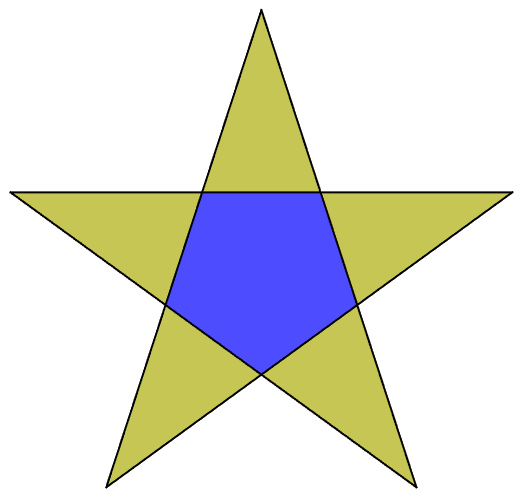
\includegraphics[width=\linewidth]{fig1a}
		\caption{In $\left\{\frac{5}{2}\right\}$}
		\end{subfigure}
		\begin{subfigure}[t]{0.4\linewidth}
			\centering
			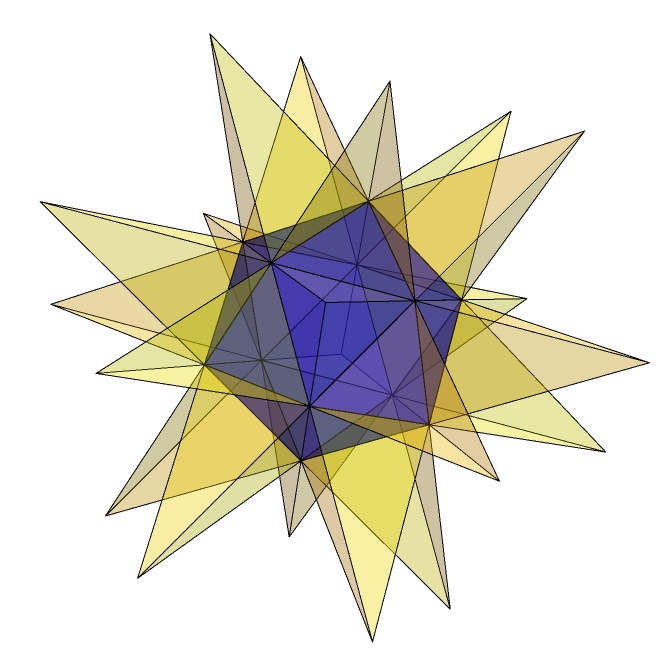
\includegraphics[width=\linewidth]{fig1b}
			\caption{In $\left\{\frac{5}{2},3\right\}$}
		\end{subfigure}
		\end{center}
		\caption{Polytopes of false vertices.}\label{fig:1}
	\end{figure}
	
	This icosahedron is thought to be the vertex figure of some vertex in $\{3,3,5\}$, so that its center and its vertices represent some vertices of $\{3,3,5\}$. We choose a base flag for this icosahedron, which determines the generating reflections $R_0$ to $R_3$ of the group $[3,3,5]$. Then we choose a base flag in the surrounding $\left\{\frac{5}{2},3\right\}$, which determines reflections $P_0$ to $P_3$. We show how to express the $P_i$ in terms of the $R_i$. Acting with the group generated by the $P_i$ on the base flag of  $\left\{\frac{5}{2},3\right\}$ will generate $\left\{\frac{5}{2},3,5\right\}$.
	
	\subsection{3-dimensional analogue}
	
	For better understanding, we start by presenting the 3-dimensional analogue of our argument. Take the pentagon of false-vertices of the pentagram to be the vertex-figure of some vertex in a regular icosahedron $\{3,5\}$, and choose a base flag for the icosahedron. We represent such flag by the \textit{basic tetrahedron} given by the base vertex and the centroids of the base edge, the base face and the icosahedron (\cref{fig:2b}). To it corresponds a triangle shown in \cref{fig:2a}.
	
	\begin{figure}[H]
		\begin{center}
			\begin{subfigure}{0.4\linewidth}
				\centering
				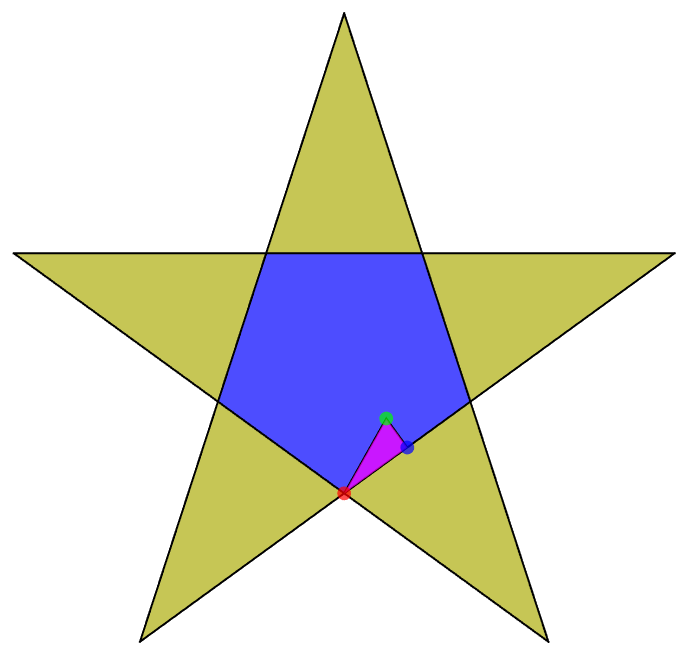
\includegraphics[width=\linewidth]{fig2a}
				\caption{Seen in $\left\{\frac{5}{2}\right\}$}\label{fig:2a}
			\end{subfigure}
			\begin{subfigure}{0.4\linewidth}
				\centering
				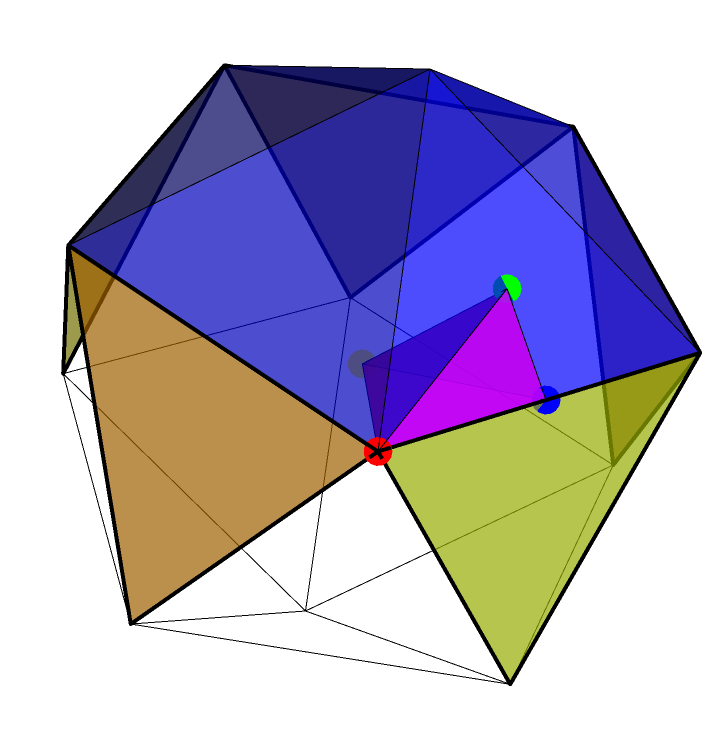
\includegraphics[width=\linewidth]{fig2b}
				\caption{Seen in $\{3,5\}$}\label{fig:2b}
			\end{subfigure}
		\end{center}
		\caption{Base flag of $\{3,5\}$.}\label{fig:2}
	\end{figure}
	
	We denote reflections and their mirrors with the same symbol. Let $R_i$ for $i=0,1,2$ be reflections on the sides of the triangle in \cref{fig:2a} in the following way: $R_0$ goes through the blue and green vertex, $R_1$ through the red and blue, and $R_2$ through the red and green. Notice these lines correspond to planes through the origin in \cref{fig:2b}, so that the $R_i$ may be thought as plane reflections.
	
	Now choose a flag for the pentagram in the 2-dimensional picture as represented in \cref{fig:3a}. We define the reflections $P_i$ on the sides of this triangle in terms of the $R_i$ as follows:
	
	\[P_0=R_0,\qquad P_1=R_1R_2R_1R_0R_1R_2R_1\qquad\text{and}\qquad P_2=R_2.\]
	
	$P_1$ is just conjugating $R_0$ by the reflection through the vertical line in the center of the picture. Like before, we may think the $P_i$ are plane reflections.
	
	If the group $\langle P_0,P_1,P_2\rangle$ is a C-string group, then it is an abstract polytope, and finding a geometric realization by Wythoff's construction amounts to finding a vertex fixed by $P_1$ and $P_2$ but not by $P_0$.
	\begin{figure}[H]
		\begin{center}
			\begin{subfigure}{0.4\linewidth}
				\centering
				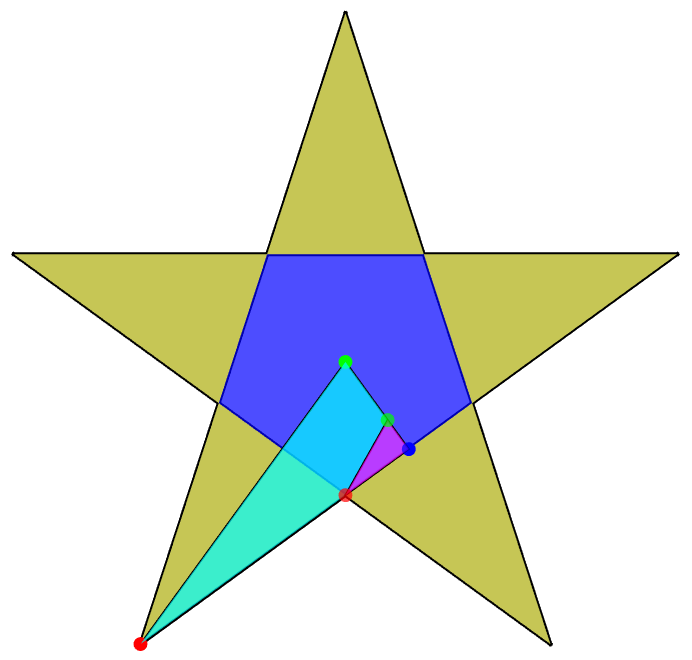
\includegraphics[width=\linewidth]{fig3a}
				\caption{Seen in $\left\{\frac{5}{2}\right\}$}\label{fig:3a}
			\end{subfigure}
			\begin{subfigure}{0.4\linewidth}
				\centering
				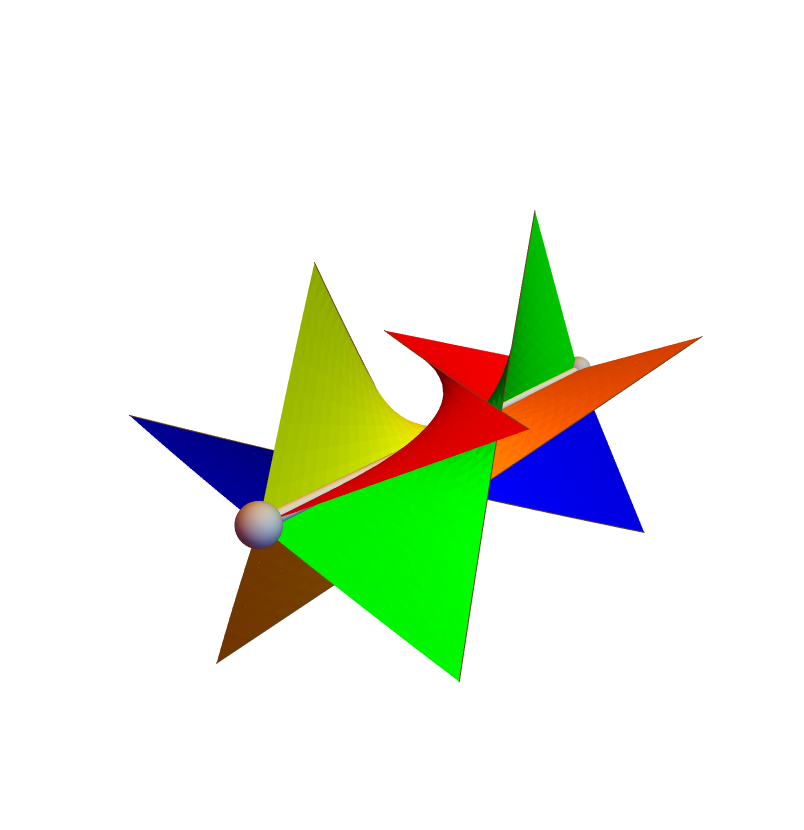
\includegraphics[width=\linewidth]{fig3b}
				\caption{Seen in $\{3,5\}$}\label{fig:3b}
			\end{subfigure}
		\end{center}
		\caption{Base flag of $\left\{\frac{5}{2}\right\}$.}\label{fig:3}
	\end{figure}
	
	For the natural choice of base vertex in our construction, we obtain a base flag (\cref{fig:3b}) as explained in \Cref{subsec:realizations}. Upon acting with the whole group on this flag, we produce $\left\{\frac{5}{2},5\right\}$, a regular star polyhedron with the same vertex-set as the icosahedron (\cref{fig:4}).
	
	\begin{figure}[H]
		\centering
		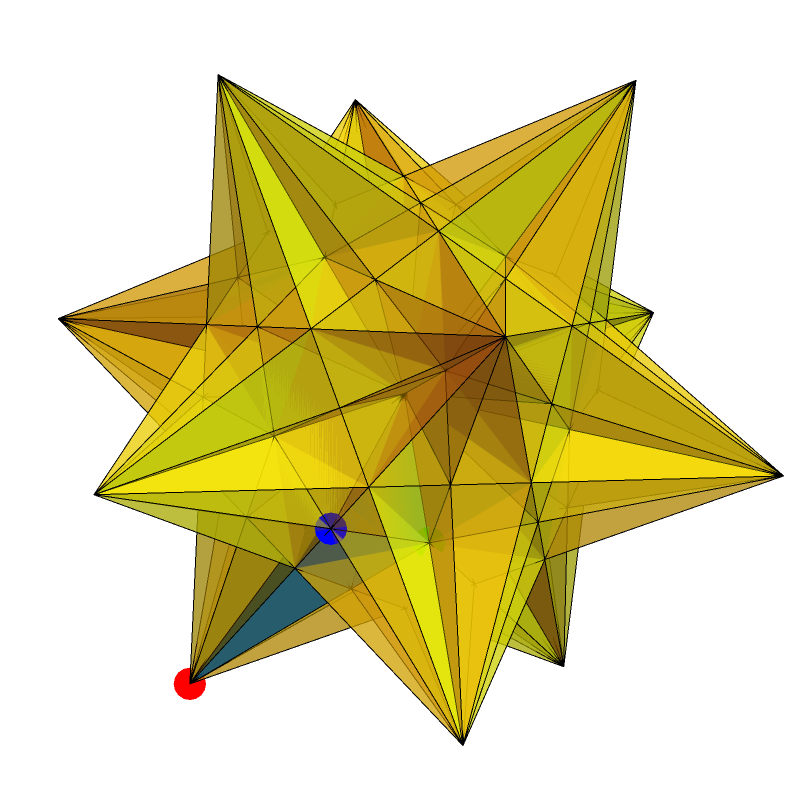
\includegraphics[width=.5\linewidth]{fig4}
		\caption{$\left\{\frac{5}{2},5\right\}$.}\label{fig:4}
	\end{figure}
	
	
	\subsection{Construction of $\left\{\frac{5}{2},3,5\right\}$ from $\{3,3,5\}$}
	
	Now we take the icosahedron of false vertices within $\left\{\frac{5}{2},3\right\}$ to be the vertex-figure of some vertex in $\{3,3,5\}$, and we choose a base flag for $\{3,3,5\}$. Recall the cells of $\{3,3,5\}$ are tetrahedra, and notice our choice of base flag does not contain the vertex of which $\{3,5\}$ is thought to be the vertex-figure (\cref{fig:5a,fig:5b}).

	\begin{figure}[H]
		\begin{center}
			\begin{subfigure}{0.49\linewidth}
				\centering
				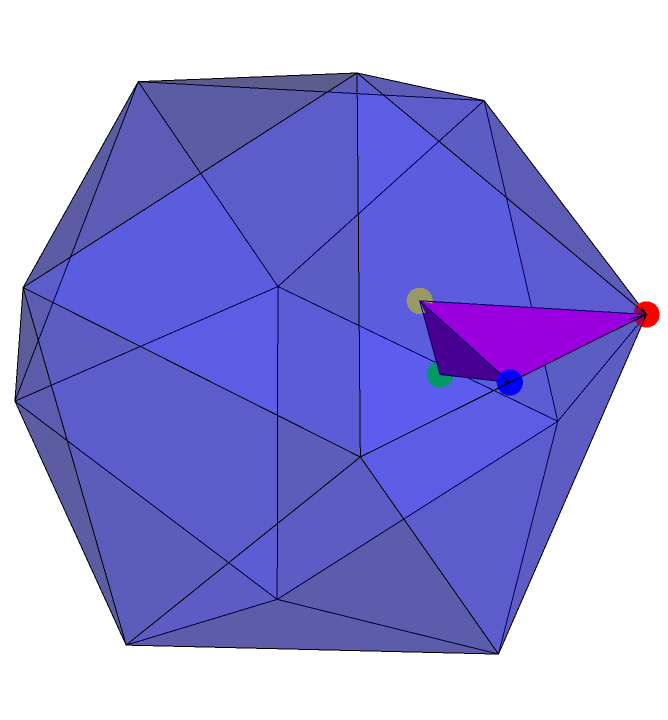
\includegraphics[width=0.9\linewidth]{fig5a}
				\caption{In $\{3,5\}$.}\label{fig:5a}
			\end{subfigure}
			\begin{subfigure}{0.49\linewidth}
				\centering
				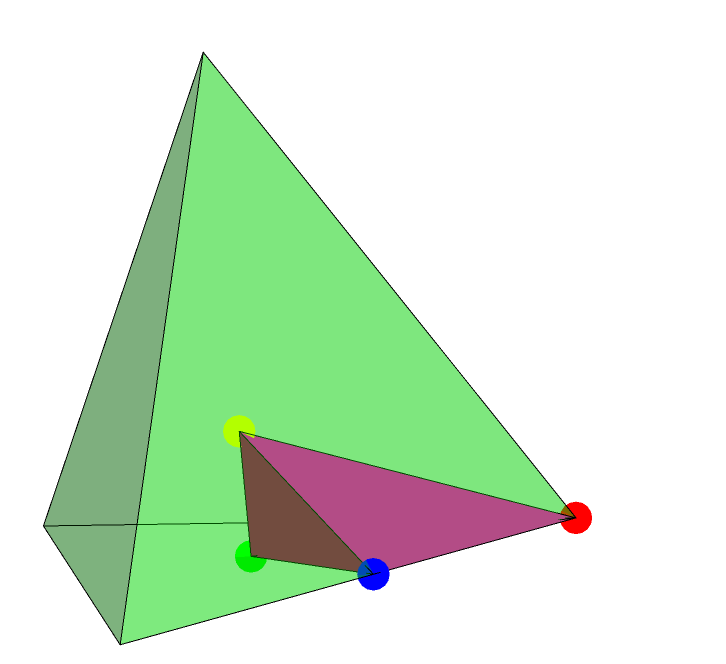
\includegraphics[width=0.9\linewidth]{fig5b}
				\caption{In the base cell.}\label{fig:5b}
			\end{subfigure}
		\end{center}
		\caption{Base flag of $\{3,3,5\}$.}\label{fig:5}
	\end{figure}
	Next we choose a base flag for $\left\{\frac{5}{2},3\right\}$ (\cref{fig:6a,fig:6b}).
	
		\begin{figure}[H]
		\begin{center}
			\begin{subfigure}{.8\linewidth}
				\centering
				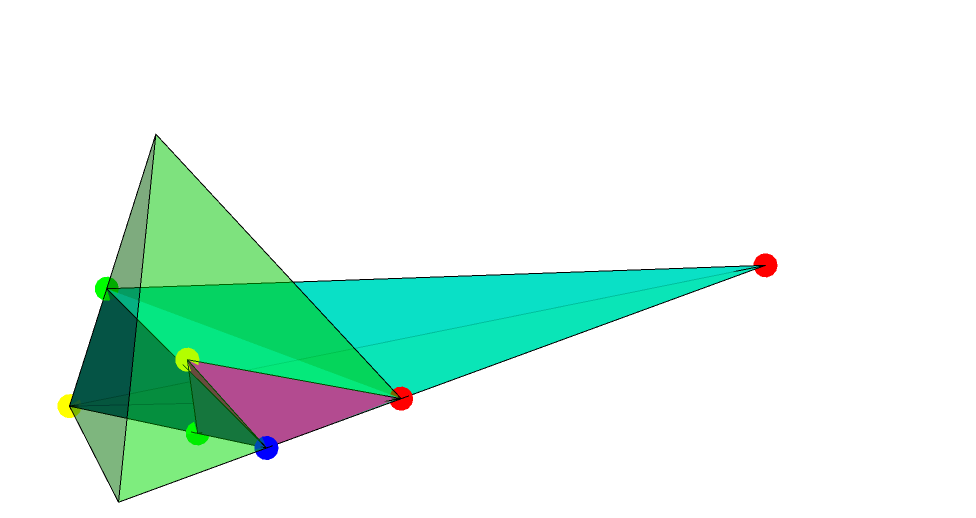
\includegraphics[width=0.9\linewidth]{fig6a}
				\subcaption{In the base cell of $\{3,3,5\}$.}\label{fig:6a}
			\end{subfigure}
			\caption{Base flags of $\{3,3,5\}$ and $\left\{\frac{5}{2},3\right\}$.}
		\end{center}
		\end{figure}

	
		\begin{figure}[H]\ContinuedFloat
		\begin{center}
			\begin{subfigure}{0.8\linewidth}
				\centering
				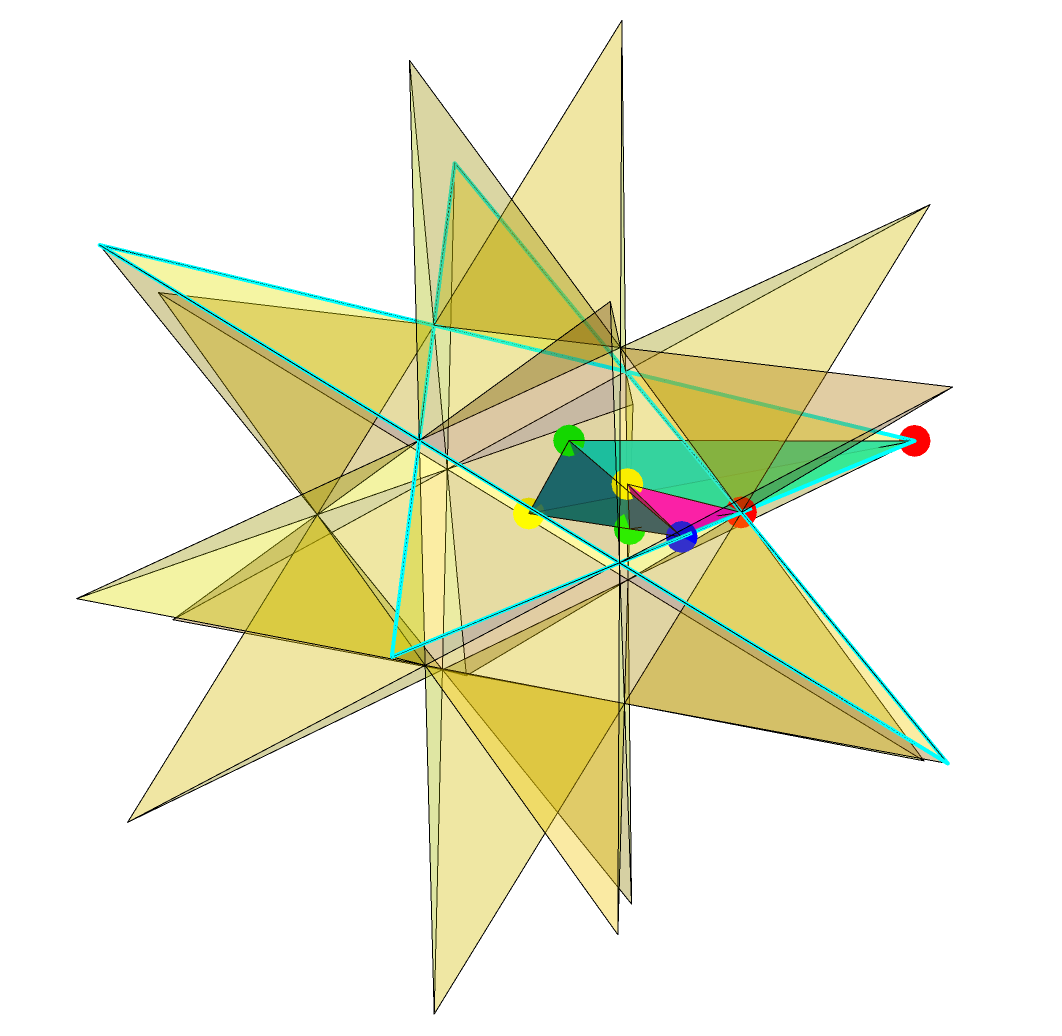
\includegraphics[width=0.9\linewidth]{fig6b}
				\subcaption{In $\left\{\frac{5}{2},3\right\}$. Edges in the base face of $\left\{\frac{5}{2},3\right\}$ are highlighted.}\label{fig:6b}
			\end{subfigure}
		\end{center}
		\caption{Base flags of $\{3,3,5\}$ and $\left\{\frac{5}{2},3\right\}$.}
	\end{figure}
%	\begin{figure}[H]
%		\centering
%		\includegraphics[width=.45\linewidth]{fig6}
%		\caption{Base flags of $\{3,3,5\}$ and $\left\{\frac{5}{2},3\right\}$.}\label{fig:6}
%	\end{figure}
	
	We may define the generating reflections of the symmetry group of $\{3,3,5\}$ using its base flag as follows. Define the red vertex as $v_0$, the blue $v_1$, the green $v_2$ and the yellow $v_3$. The mirror of the reflection $R_i$ is the plane through all but $v_i$ (as an example we show $R_0$ in \cref{fig:7}).
	
	\begin{figure}[H]
		\centering
		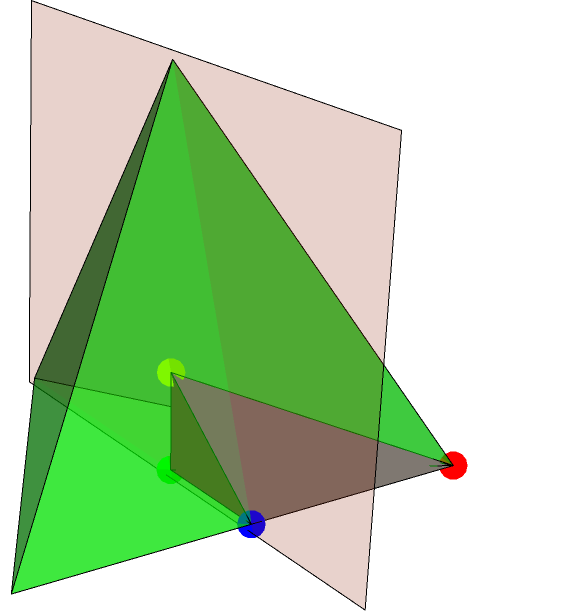
\includegraphics[width=.3\linewidth]{fig7}
		\caption{$R_0$.}\label{fig:7}
	\end{figure}
	
	Recall we think of these as hyperplane reflections, each determined by three vertices in the base flag and the origin in 4-space.
	
	Now we may define the generatig reflections for the symmetry group of $\left\{\frac{5}{2},3,5\right\}$ in terms of the $R_i$ (\cref{fig:8}).
	
	\begin{figure}[H]
	\begin{center}
		\begin{subfigure}{\linewidth}
				\centering
				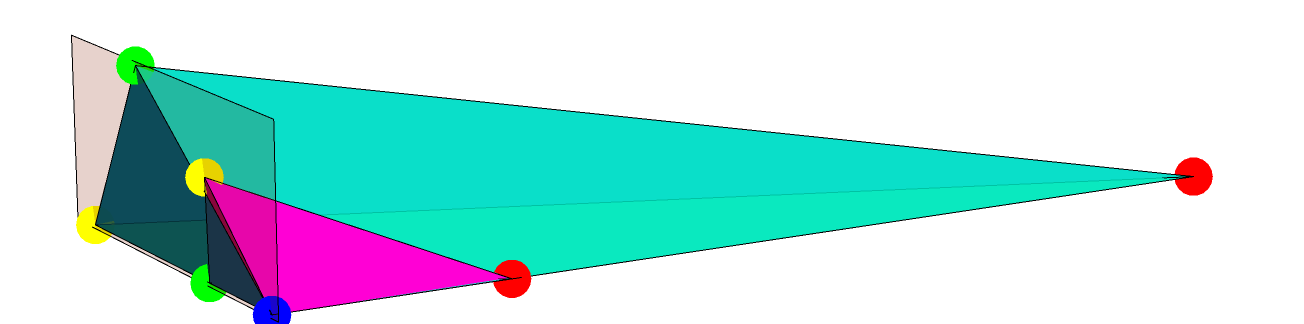
\includegraphics[width=0.95\linewidth]{fig8a}
				\caption{$P_0=R_0$.}\label{fig:8a}
		\end{subfigure}
		
		\begin{subfigure}{\linewidth}
			\centering
			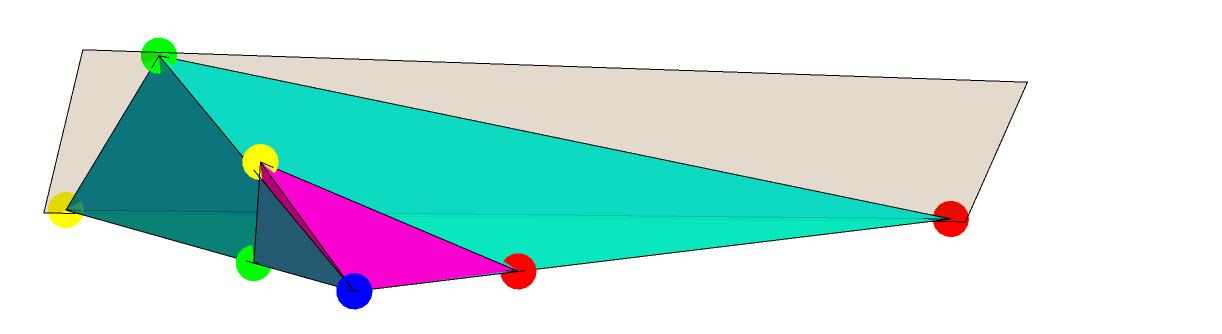
\includegraphics[width=0.95\linewidth]{fig8b}
			\caption{$P_1=R_1R_2R_3R_2R_1R_0R_1R_2R_3R_2R_1$.}\label{fig:8b}
		\end{subfigure}
		
		\begin{subfigure}{\linewidth}
				\centering
				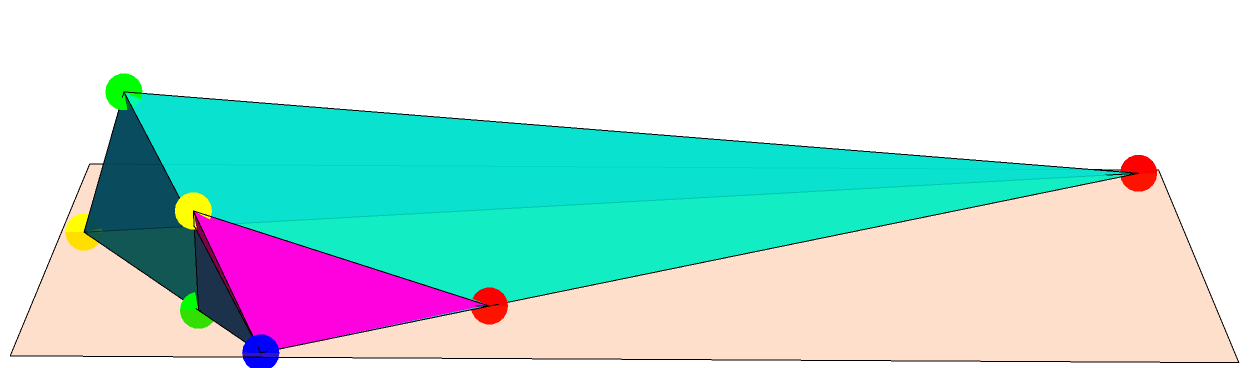
\includegraphics[width=0.95\linewidth]{fig8c}
				\caption{$P_2=R_3$.}\label{fig:8c}
		\end{subfigure}
		
		\begin{subfigure}{\linewidth}
			\centering
			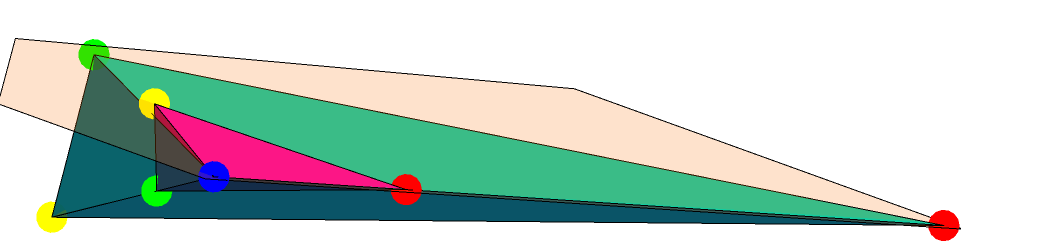
\includegraphics[width=0.95\linewidth]{fig8d}
			\caption{$P_3=R_2$.}\label{fig:8d}
		\end{subfigure}
		\end{center}
		\caption{The $P_i$ in terms of the $R_i$.}\label{fig:8}
	\end{figure}
	
	$P_1$ is just $R_0$ conjugated by $R_1R_2R_3R_2R_1$ (\cref{fig:9a,fig:9b}).
	
	\begin{figure}[H]
	\begin{center}
		\begin{subfigure}{\linewidth}
			\centering
			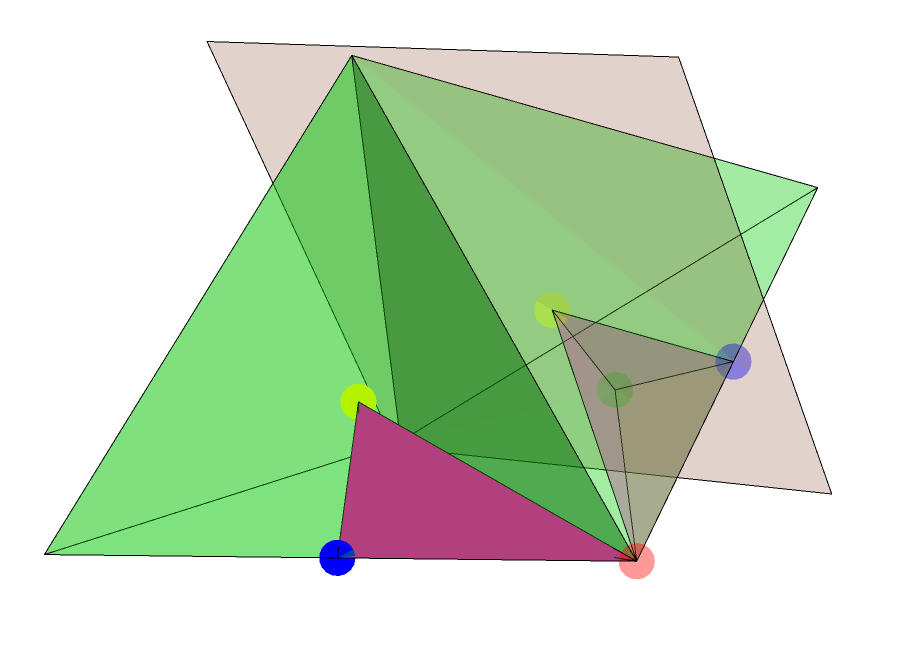
\includegraphics[width=0.5\linewidth]{fig9a}
			\caption{$R_0$ conjugated by $R_1R_2R_3R_2R_1$.}\label{fig:9a}
		\end{subfigure}
		\begin{subfigure}{\linewidth}
			\centering
			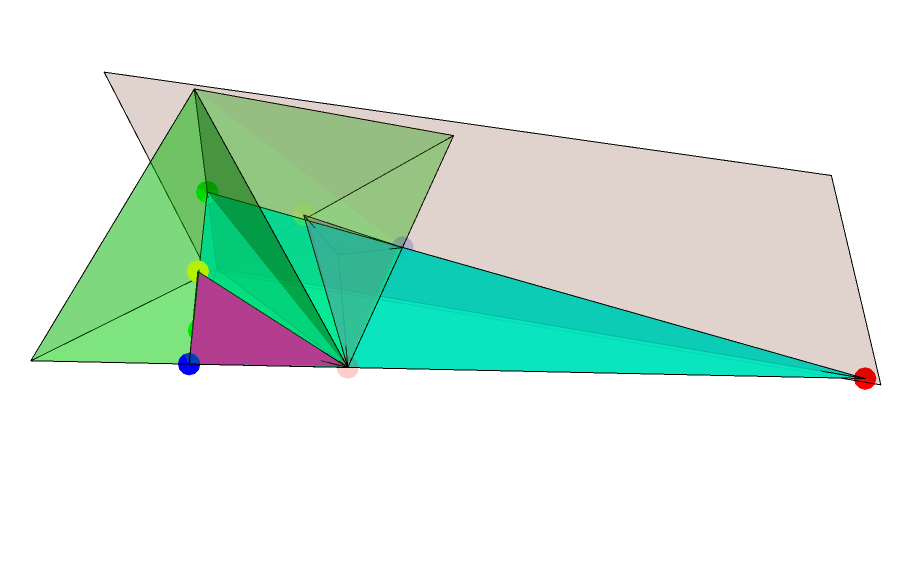
\includegraphics[width=0.9\linewidth]{fig9b}
			\caption{Showing the base flag of $\left\{\frac{5}{2},3\right\}$.}\label{fig:9b}
		\end{subfigure}
		\end{center}
		\caption{$P_1$.}
		\end{figure}
	
	It has been confirmed in \texttt{abstract.txt} that $\langle P_0,P_1,P_2,P_3\rangle$ is a C-string group (see \Cref{app:1}). Specifically,
		\[P_i^2=(P_0P_1)^5=(P_1P_2)^3=(P_2P_3)^5=(P_0P_2)^2=(P_0P_3)^2=(P_1P_3)^2=\Id\]
	for all $i$, and the intersection property holds (see \texttt{int-prop.txt}).
	

	To produce a realization we must find a vertex fixed by $P_1$, $P_2$ and $P_3$ but not by $P_0$. The natural choice is shown in \cref{fig:10}, and it is defined as follows. First we take $v_0$ to the opposite vertex of the base face in the base tetrahedron using $R_0R_1R_2$. Next we rotate twice about the base edge conjugated by $R_1R_2R_3R_2R_1$.
	
		\begin{figure}[H]
		\begin{center}
			\begin{subfigure}{\linewidth}
				\centering
				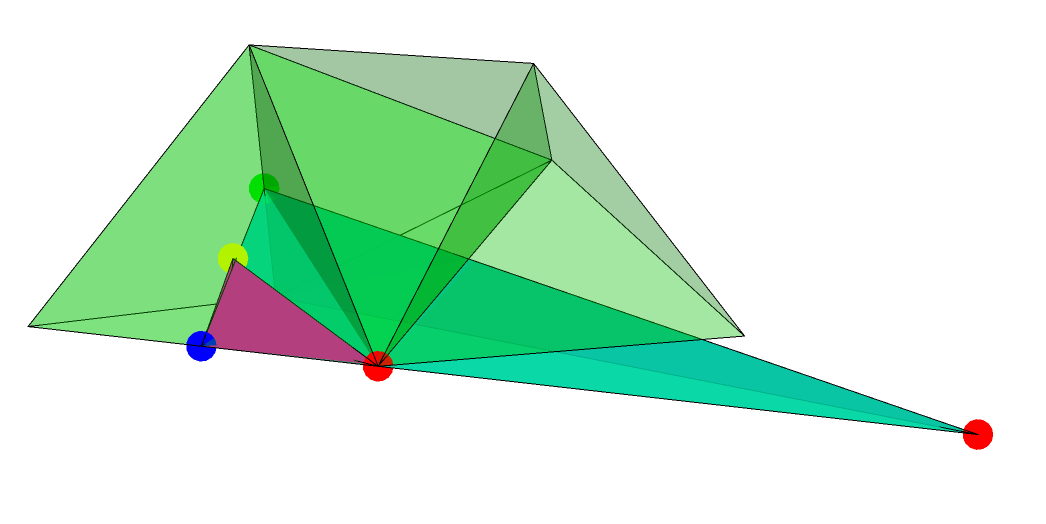
\includegraphics[width=0.8\linewidth]{fig10a}
				\caption{As we've been picturing it.}\label{fig:10a}
			\end{subfigure}
			\begin{subfigure}{\linewidth}
				\centering
				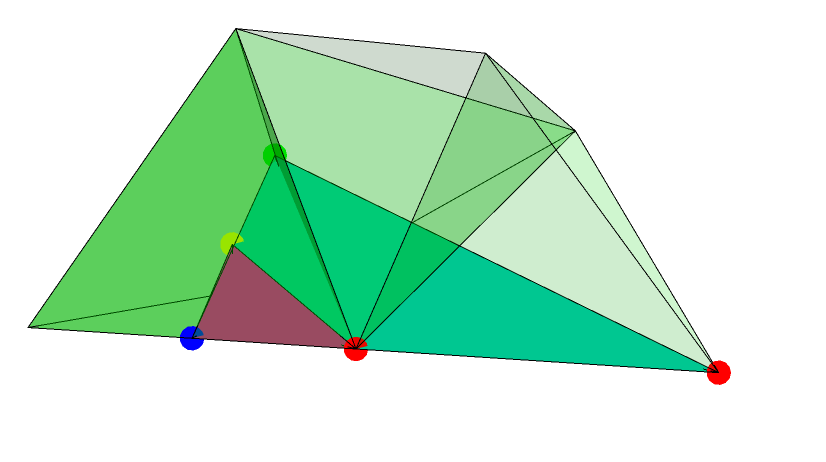
\includegraphics[width=0.7\linewidth]{fig10b}
				\caption{Stereographic projection.}\label{fig:10b}
			\end{subfigure}
		\end{center}
		\caption{The base vertex of $\left\{\frac{5}{2},3,5\right\}$.}\label{fig:10}
	\end{figure}
	
	So let
		\begin{equation}\label{eq:w0}
			w_0:=v_0R_0R_1R_2\cdot R_1R_2R_3R_2R_1\cdot  R_3R_2R_3R_2\cdot R_1R_2R_3R_2R_1,
		\end{equation}
	(we use dots to facilitate lecture), which is, in effect, fixed by all $P_i$ but $P_0$ (see \texttt{geometric.txt}, \Cref{app:2}). We have also shown that $\langle R_0,R_1,R_2,R_3\rangle=\langle P_0,P_1,P_2,P_3\rangle$, so that the vertex-set in both structures is the same (this equality also follows from thm. 7D13, \cite{abstract-polytopes}). It follows that the realization is symmetric. Faithfulness was proved by comparing the number of $i$-faces in \texttt{abstract.txt} and \texttt{geometric.txt}.
	
	Since the $R_i$ are hyperplane reflections, we have a classical polytope as defined in \Cref{subsec:realizations} (see \cite{mcmullen-4dimensional}). The only such polytopes in $\mathbb{E}^4$ arising from the regular abstract polytope$\{5,3,5\}$ are the star 4-polytopes $\left\{\frac{5}{2},3,5\right\}$ and $\left\{5,3,\frac{5}{2}\right\}$ (thm. 7D13 \cite{abstract-polytopes}). However, the rotation about the edge in this polytope is the reverse of that of the $\{3,3,5\}$, so it cannot be of type $\frac{5}{2}$. This completes the proof that we have constructed $\left\{\frac{5}{2},3,5\right\}$.
	
	\begin{figure}[H]
		\begin{center}
			\begin{subfigure}{\linewidth}
				\centering
				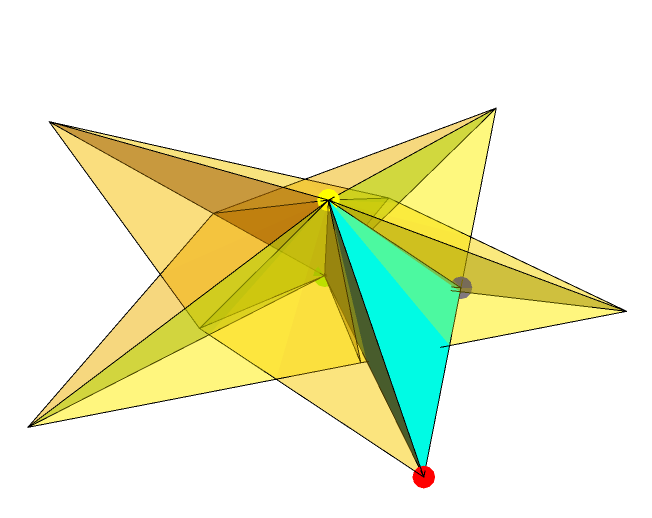
\includegraphics[width=0.5\linewidth]{fig11a}
				\caption{The base face.}\label{fig:11a}
			\end{subfigure}
			\begin{subfigure}{\linewidth}
				\centering
				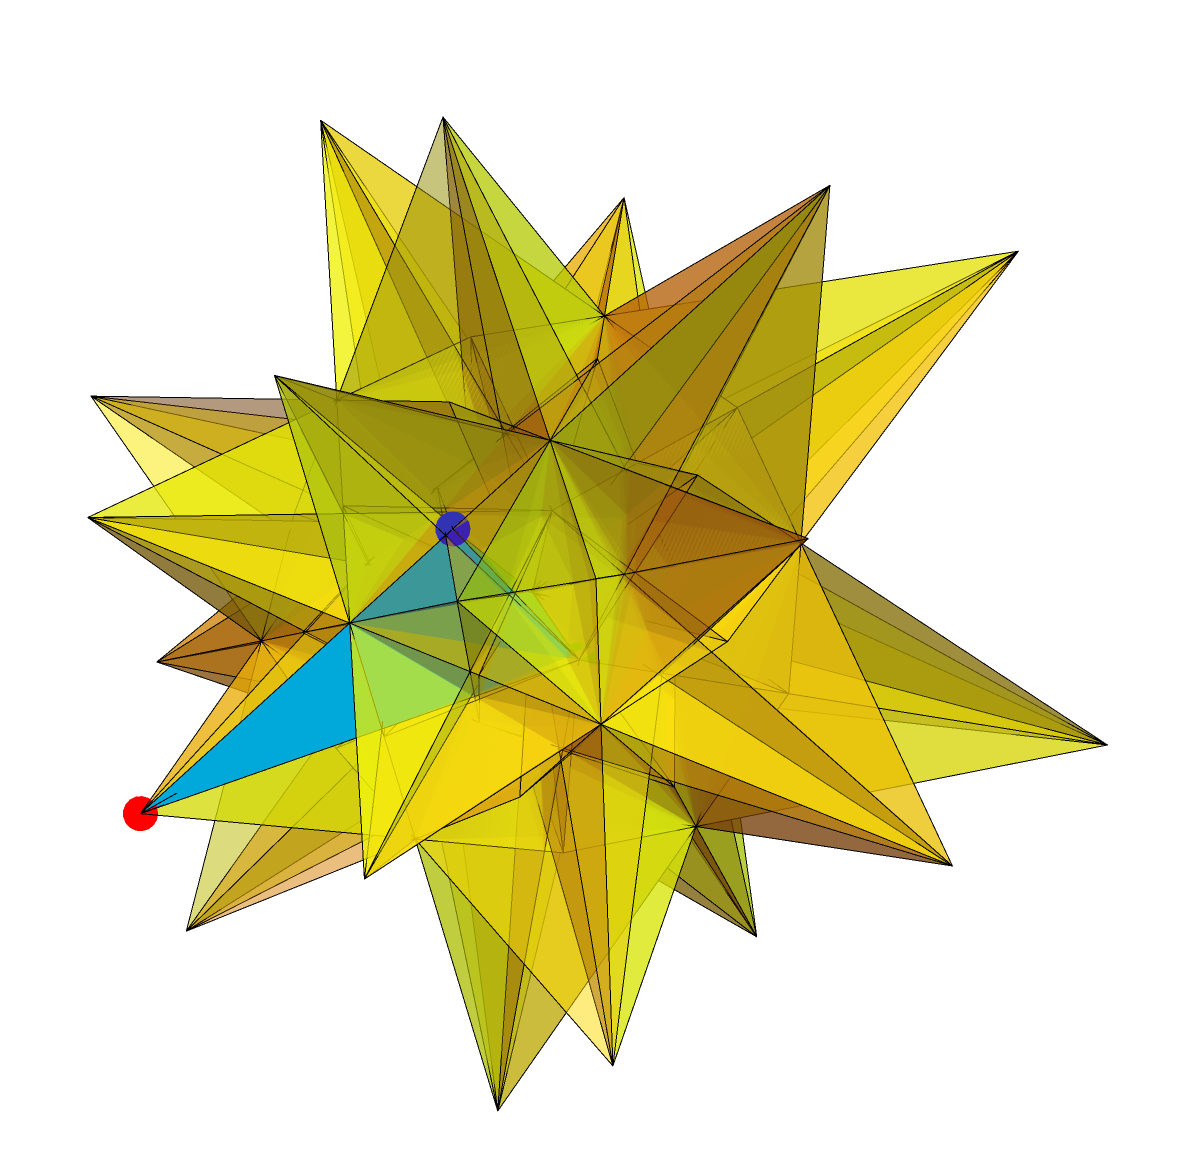
\includegraphics[width=0.7\linewidth]{fig11b}
				\caption{The base cell.}\label{fig:11b}
			\end{subfigure}
		\end{center}
		\caption{Stereographic projections of  $\left\{\frac{5}{2},3,5\right\}$.}\label{fig:11}
	\end{figure}

	\section{A chiral 4-polytope from $\left\{\frac{5}{2},3,5\right\}$}
	To construct a chiral 4-polytope we must define the generating rotations. From the given realization of $\left\{\frac{5}{2},3,5\right\}$, let
		\[S_1=P_0P_1P_3P_2,\qquad S_2=P_2P_1,\quad\text{and}\quad S_3=P_3P_2.\]
	It is shown in \texttt{abstract.txt} that
		\[S_1^{12}=S_2^3=S_3^5=(S_1S_2)^2=(S_1S_2S_3)^2=(S_2S_3)^2=\Id\]
	and that the intersection property holds, so that the group may be thought as a regular or chiral abstract polytope. For a realization by Wythoff's construction define the base vertex to be the same $w_0$ that was used for $\left\{\frac{5}{2},3,5\right\}$. Since the base vertex is the same for both structures, and the group $\langle S_1,S_2,S_3\rangle$ is a subgroup of $\langle P_0,P_1,P_2,P_3\rangle$, it follows that the realization is symmetric. Again, by comparing the number of $i$-faces in \texttt{abstract.txt} and \texttt{geometric.txt} our realization is seen to be faithful.
	
	The choices of $S_1$ and $S_2$ are as in  \cite{petcox}, so that the cells are copies of the chiral polyhedron denoted as $H_1(\left\{5,3,\frac{5}{2}\right\})$. In fact, chirality in our 4-polytope follows from the chirality of the cells, since any symmetry sending a flag to its $i$-th adjacent is also a symmetry of the cell.
	
	In \texttt{geometric.txt} we have shown this structure to have 120 vertices, 720 edges, 300 faces and 50 cells. The first two numbers are the same for the regular $\left\{\frac{5}{2},3,5\right\}$, meaning the vertex and edge-sets are the same for both polytopes. Every face has 12 vertices and edges arranged in helical fashion as shown in \cite{petcox} (see \cref{fig:12}). In virtue of such arrangement we denote this polytope by $\left\{\frac{12}{1,5},3,5\right\}$.
	
	
	We now show this structure satisfies \textit{(i)-(iv)} in our definition of 4-polytope. By the realization being faithful and symmetric, conditions \textit{(i)} and \textit{(ii)} follow from (P4) and (P3), respectively.
	
	We may also show \textit{(i)} in a slightly more geometric way. It has been shown in  \texttt{geometric.txt} that for the base face $f$,
	\begin{equation*}\label{ec:stab-face}
		\Stab_{\langle S_1,S_2,S_3\rangle}(f)=\langle S_1,S_2S_3\rangle,
	\end{equation*}
	which implies that every face belongs to exactly two cells. This follows since $S_1$ fixes the base cell and $S_2S_3$ an involution. If any cell has $f$ as a face, we may map it to the base cell by a transformation fixing $f$.
	
	 For \textit{(iii)} notice the vertex figures are icosahedra. This follows from Wythoff's construction on any vertex adjacent to the base vertex by the group $\langle S_2,S_3\rangle$. Finally, \textit{(iv)} is immediate from the finiteness of the group. This concludes the proof that we have produced a chiral 4-polytope.
	
	Further, it was found in \texttt{abstract.txt} that there exists no automorphism $\rho$ of the group generated by the $S_i$ that satisfies \cref{eq:combinatorially-chiral}, so that the abstract polytope associated to $\left\{\frac{12}{1,5},3,5\right\}$ is still chiral.
	
	

\begin{figure}[H]
	\begin{center}
%		\begin{subfigure}{\linewidth}
			\centering
			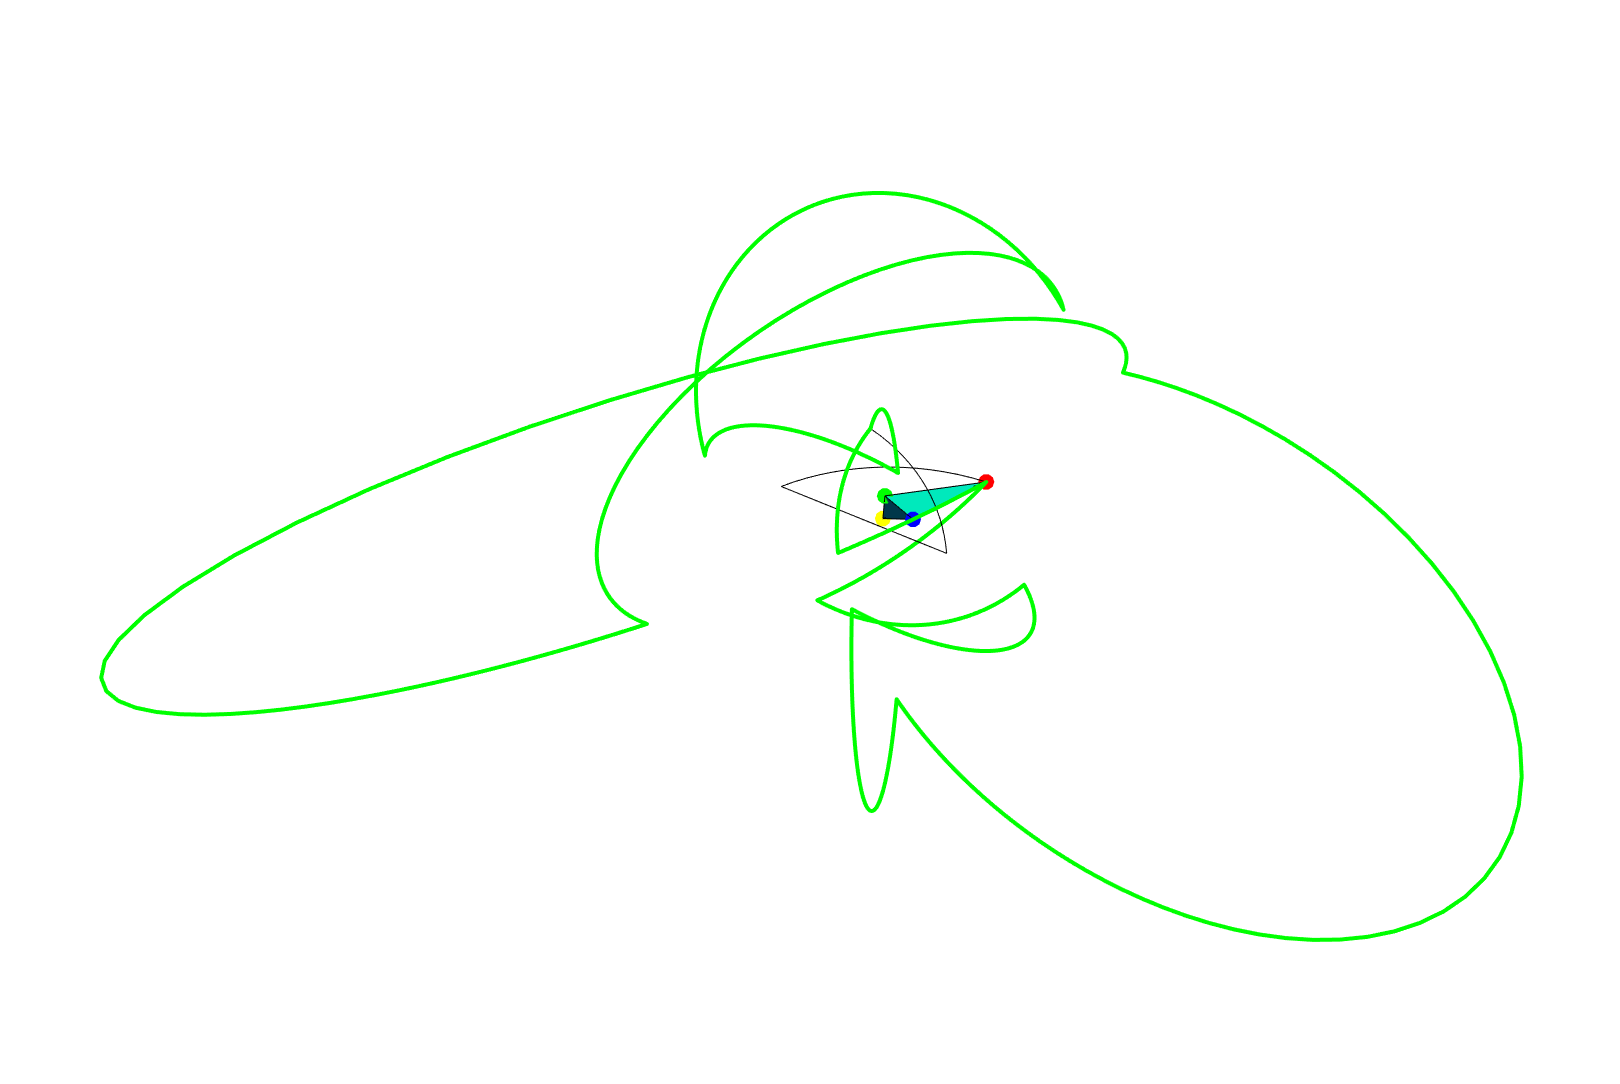
\includegraphics[width=1\linewidth]{fig12a}
%			\caption{The base face. We also show the base face and flag of $\left\{\frac{5}{2},3,5\right\}$}\label{fig:12a}
%		\end{subfigure}
%		\begin{subfigure}{\linewidth}
%			\centering
%			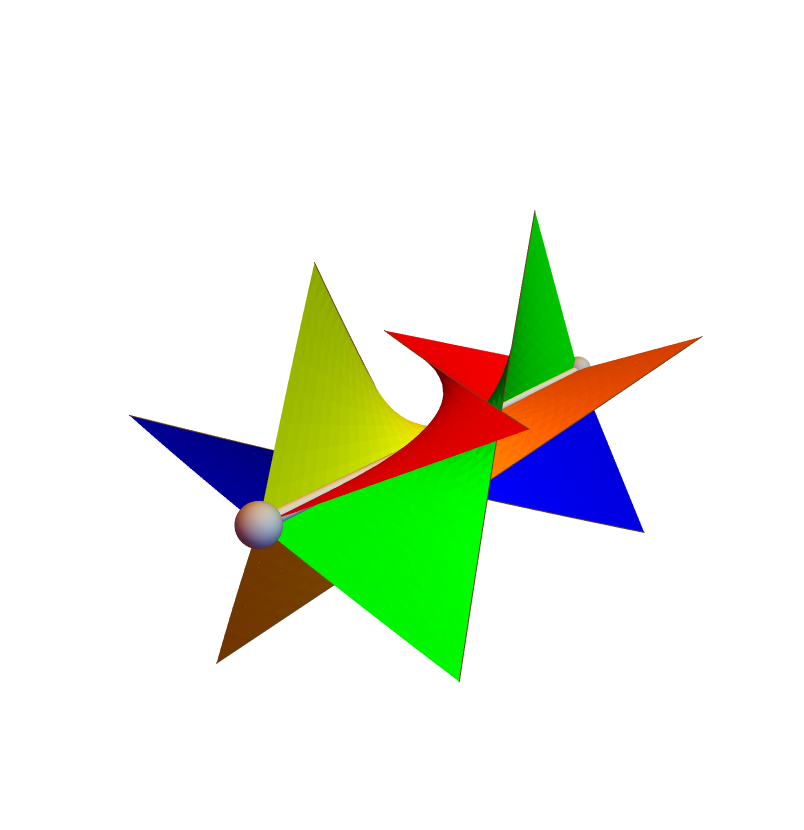
\includegraphics[width=0.5\linewidth]{fig12b}
%			\caption{Five faces at the edge. We show part of the surface spanned between the edge and the axis of twist in every face.}\label{fig:12b}
%		\end{subfigure}
	\end{center}
	\caption{Stereographic projection of the base face of  $\left\{\frac{12}{1,5},3,5\right\}$. We also show the base face and flag of $\left\{\frac{5}{2},3,5\right\}$}\label{fig:12}
\end{figure}

	
	\section{A chiral 4-polytope from $\left\{5,3,\frac{5}{2}\right\}$}
	For the dual star polytope $\left\{5,3,\frac{5}{2}\right\}$ we simple define
	\[Q_0=P_3,\qquad Q_1=P_2\qquad Q_2=P_3,\quad\text{and}\quad Q_3=P_0\]
	and apply Wythoff's construction on the centroid of the base cell of the $\left\{\frac{5}{2},3,5\right\}$. The coordinates of this point were computed in \texttt{geometric-dual.txt}.
	
	Analogue definitions to those of the $S_i$ produce another chiral 4-polytope with the same properties as the former; namely, number of vertices, edges, faces and cells, and combinatorial chirality. Every step of the construction was confirmed in \texttt{abstract-dual.txt} and \texttt{geometric-dual.txt} (and \texttt{int-prop-dual.txt}).
	
	In this case, the cells are copies of $H_0(\left\{5,3,\frac{5}{2}\right\})$ from \cite{petcox}. We call it $\left\{\frac{12}{1,5},3,\frac{5}{2}\right\}$.
	
\begin{figure}[H]
	\begin{center}
		\begin{subfigure}{\linewidth}
			\centering
			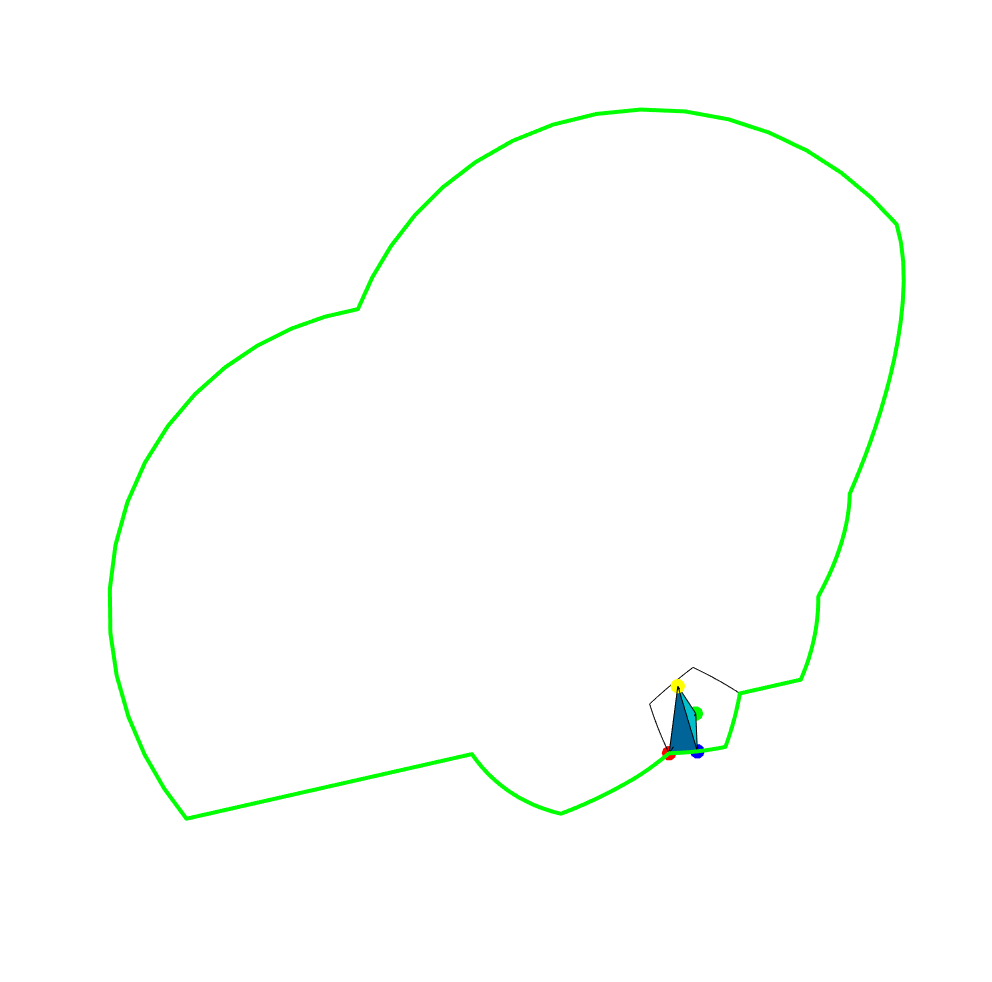
\includegraphics[width=0.7\linewidth]{fig13a}
			\caption{The base face. We also show the base face and flag of $\left\{5,3,\frac{5}{2}\right\}$}\label{fig:13a}
		\end{subfigure}
		\begin{subfigure}{\linewidth}
			\centering
			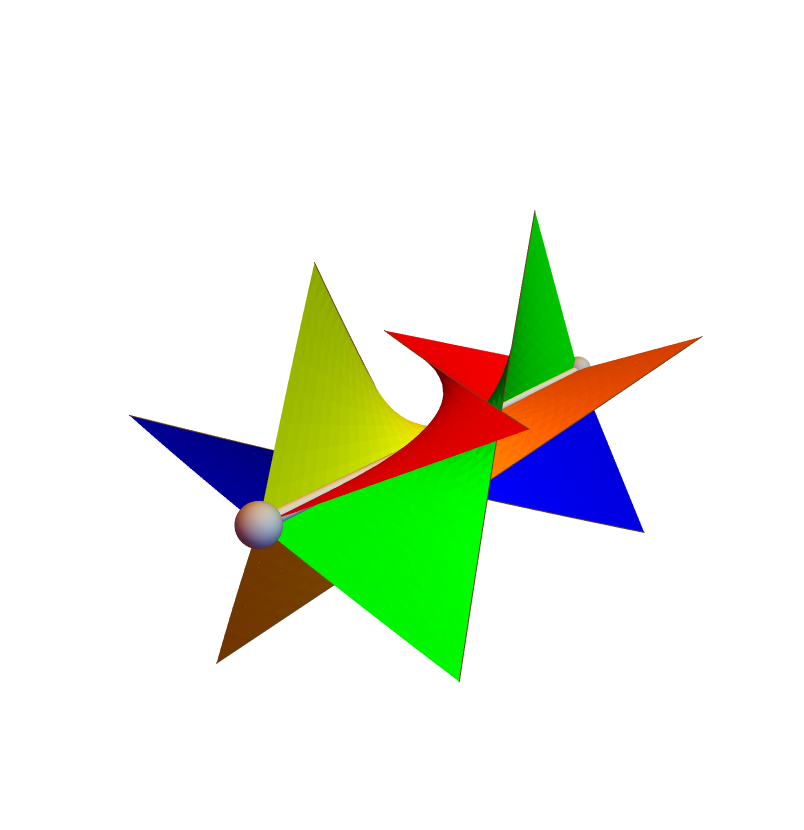
\includegraphics[width=0.5\linewidth]{fig12b}
			\caption{Five faces at the edge. We show part of the surface spanned between the edge and the axis of twist in every face.}\label{fig:13b}
		\end{subfigure}
	\end{center}
	\caption{Stereographic projections of  $\left\{\frac{12}{1,5},3,\frac{5}{2}\right\}$.}\label{fig:13}
\end{figure}

\clearpage
\begin{appendices}
\crefalias{subsection}{appendix}
\section{GAP programs}
In the following sections we show the output of the files \texttt{abstract.txt} and \texttt{geometric.txt} as executed in GAP. The original code for these and other programs used in this thesis may be consulted \href{https://github.com/danimalabares/tesina}{here}.

\subsection{\texttt{abstract.txt}}\label{app:1}

\begin{changemargin}{-2cm}{-2cm}
\begin{multicols}{2}
\begin{lstlisting}
	-------------------------------
	ABSTRACT POLYTOPES
	-------------------------------
	
	-------------------------------
	STRING RELATIONS OF {5/2,3,5}
	|<P0>|=2
	|<P1>|=2
	|<P2>|=2
	|<P3>|=2
	
	|<P0*P1>|=5
	|<P1*P2>|=3
	|<P2*P3>|=5
	
	|<P0*P2>|=2
	|<P0*P3>|=2
	|<P1*P3>|=2
	
	Are the groups of {3,3,5} and {5/2,3,5} the same? true
	
	
	-------------------------------
	FACE COUNT OF THE THREE POLYTOPES
	
	{3,3,5}
	
	Vertices in the face: 3
	Vertices in the cell: 4
	Vertices in the polytope: 120
	Edges in the face: 3
	Edges in the cell: 6
	Edges in the polytope: 720
	Faces in the cell: 4
	Faces in the polytope: 1200
	Cells in the polytope: 600
	
	
	{5/2,3,5}
	
	Vertices in the face: 5
	Vertices in the cell: 20
	Vertices in the polytope: 120
	Edges in the face: 5
	Edges in the cell: 30
	Edges in the polytope: 720
	Faces in the cell: 12
	Faces in the polytope: 720
	Cells in the polytope: 120
	
	
	Chiral
	
	Vertices in the cell: 48
	Vertices in the polytope: 120
	Edges in the cell: 72
	Edges in the polytope: 720
	Faces in the cell: 12
	Faces in the polytope: 300
	Cells in the polytope: 50
	
	
	-------------------------------
	STRING RELATIONS OF CHIRAL
	
	|<S1>|=12
	|<S2>|=3
	|<S3>|=5
	
	|<S1*S2>|=2
	|<S1*S2*S3>|=2
	|<S2*S3>|=2
	
	
	-------------------------------
	INTERSECTION PROPERTY OF CHIRAL
	
	<S1>INT<S2>==<1>  true
	<S2>INT<S3>==<1>  true
	<S1,S2>INT<S2,S3>==<S2>  true
	
	\end{lstlisting}
	\vfill\null\columnbreak
	\begin{lstlisting}
	-------------------------------
	COMBINATORIALLY CHIRAL
	
	Is there an automorphism that satisfies eq. (3)?
	
	rho(S1)=S1^-1  true
	rho(S2)=S1^2*S2  true
	
	Can we extend it to the whole group?  fail
\end{lstlisting}
\end{multicols}
\end{changemargin}

\subsection{\texttt{geometric.txt}}\label{app:2}
\begin{changemargin}{-2cm}{-2cm} 
\begin{multicols}{2}
\begin{lstlisting}
	-------------------------------
	GEOMETRIC POLYTOPES
	-------------------------------
	
	-------------------------------
	STRING RELATIONS OF {5/2,3,5} 
	|<P0>|=2
	|<P1>|=2
	|<P2>|=2
	|<P3>|=2
	
	|<P0*P1>|=5
	|<P1*P2>|=3
	|<P2*P3>|=5
	
	|<P0*P2>|=2
	|<P0*P3>|=2
	|<P1*P3>|=2
	
	Are the groups of {3,3,5} and {5/2,3,5} the same? true
	
	
	-------------------------------
	BASE VERTEX OF {5/2,3,5}
	
	w0P0=w0 false
	w0P1=w0 true
	w0P2=w0 true
	w0P3=w0 true
	
	-------------------------------
	FACE COUNT FOR THE THREE POLYTOPES
	
	{3,3,5}
	
	Vertices in the face: 3
	Vertices in the cell: 4
	Vertices in the polytope: 120
	Edges in the face: 3
	Edges in the cell: 6
	Edges in the polytope: 720
	Faces in the cell: 4
	Faces in the polytope: 1200
	Cells in the polytope: 600
	
	
	{5/2,3,5}
	
	Vertices in the face: 5
	Vertices in the cell: 20
	Vertices in the polytope: 120
	Edges in the face: 5
	Edges in the cell: 30
	Edges in the polytope: 720
	Faces in the cell: 12
	Faces in the polytope: 720
	Cells in the polytope: 120
	
	\end{lstlisting}
	\vfill\null\columnbreak
	\begin{lstlisting}
	
	Chiral
	
	Vertices in the face: 12
	Vertices in the cell: 48
	Vertices in the polytope: 120
	Edges in the face: 12
	Edges in the cell: 72
	Edges in the polytope: 720
	Faces in the cell: 12
	Faces in the polytope: 300
	Cells in the polytope: 50
	
	-------------------------------
	STRING RELATIONS OF CHIRAL
	|<S1>|=12
	|<S2>|=3
	|<S3>|=5
	
	|<S1*S2>|=2
	|<S1*S2*S3>|=2
	|<S2*S3>|=2
	
	
	\end{lstlisting}
	\vfill\null\columnbreak
	\begin{lstlisting}
	-------------------------------
	STABILIZERS OF CHIRAL
	
	S3 fixes the base vertex and edge?
	
	w0.S3=w0  true
	w0.S1^-1.S3=w0.S1^-1  true

	Stabilizers within the cell
	
	Stab_<S1,S2>w0=<S2>  true
	Stab_<S1,S2>e=<S1*S2>  true
	Stab_<S1,S2>f=<S1>  true
	
	
	Stabilizers within the whole polytope
	
	Stab_<S1,S2,S3>w0=<S2,S3>  true
	Stab_<S1,S2,S3>e=<S1*S2,S3>  true
	Stab_<S1,S2,S3>f=<S1,S2*S3>  true
	Stab_<S1,S2,S3>c=<S1,S2>  true
\end{lstlisting}
\end{multicols}
\end{changemargin}
\vspace{-1cm}
\section{Coordinates of geometric realizations}\label{sec:figs}
We show the coordinates as computed in \texttt{Section-5C.nb}. Let $\phi$ be the golden ratio. As in \cite{petcox}, for the basic tetrahedron of $\{3,3,5\}$
\[v_0=(1, 0, 0, 0),\quad v_1=\left(\phi+2,1,0,\frac{1}{\phi }\right), \quad v_2=\left(\phi,\frac{1}{\phi },0,0\right),\quad v_3=\left(\phi ^2,1,-\frac{1}{\phi ^2},0\right)\]
we obtain the coordinates of the base vertex of $\left\{\frac{5}{2},3,5\right\}$
\[w_0=\left(\frac{\phi }{2}, -\frac{1}{2}, 0, -\frac{1}{2 \phi }\right)\]
by defining it in as in \cref{eq:w0}. The $S_i$ for $\left\{\frac{5}{2},3,5\right\}$ have coordinates
\[
	S_1=\frac{1}{2}\left(
	\begin{array}{cccc}
		1 & 1 & 1 & -1 \\
		\phi  & -1 & 0 & \frac{1}{\phi } \\
		-\frac{1}{\phi } & -1 & \phi  & 0 \\
		0 & -1 & -\frac{1}{\phi } & -\phi  \\
	\end{array}	\right),
	\qquad S_2=\frac{1}{2}\left(
	\begin{array}{cccc}
		\phi  & 0 & -\frac{1}{\phi } & -1 \\
		0 & 2 & 0 & 0 \\
		\frac{1}{\phi } & 0 & -1 & \phi  \\
		-1 & 0 & -\phi  & -\phi{1}{\ } \\
	\end{array}
	\right),
\]\[
	S_3=\frac{1}{2}\left(
	\begin{array}{cccc}
		2 & 0 & 0 & 0 \\
		0 & \phi  & 1 & \frac{1}{\phi } \\
		0 & -1 & \frac{1}{\phi } & \phi  \\
		0 & \frac{1}{\phi } & -\phi  & 1 \\
	\end{array}
	\right)
\]

\end{appendices}
\section*{Bibliography}
\addcontentsline{toc}{section}{Bibliography}

\printbibliography[heading=none]
\end{document}